% Hamad Medical Corporation
% Georges Younes

\section{System Integration and Demonstration Prototype}\label{sec:system_integration}

\subsection{Console Setup}\label{ssec:console_setup}
We developed software with the following features:
\begin{enumerate}
  \item Able to load and render DICOM MR images, organ models (derived from MR images), and CAD models of surgical robotic instruments (which include stereoscopic camera, EndoWrist instruments, and trocars),
  \item The user can select and manipulate the positions of the trocars with Fulcrum effect simulated at the incision point (\autoref{fig:simulation_setup}), and
  \item Using the software, one can define the starting scenario for patient-specific simulation of a surgical procedure (\autoref{fig:stereoscopic_console}).
\end{enumerate}

\begin{figure}
  \centering%
  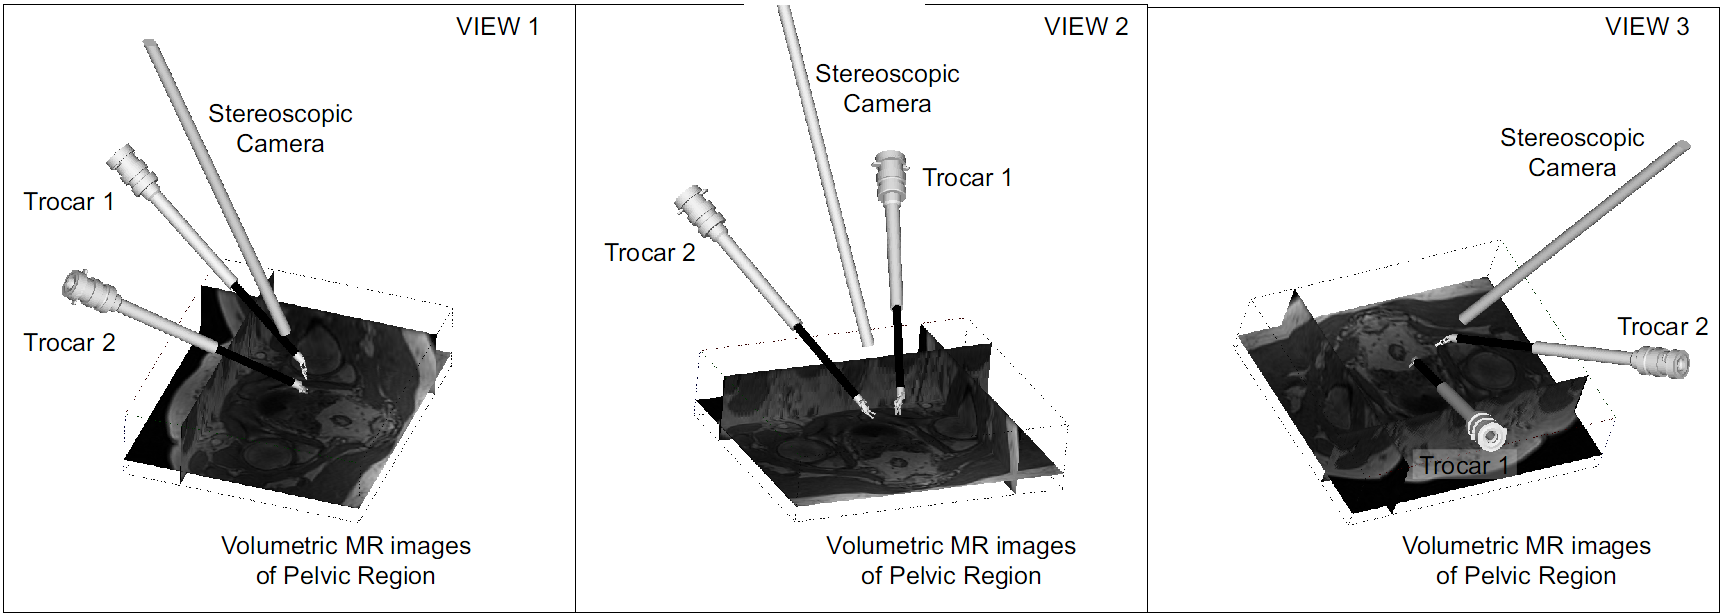
\includegraphics[width=1.0\linewidth]{integration/multiple_views_fusion}
  \caption{Simulation setup rendered by software from different viewpoints.}\label{fig:simulation_setup}
\end{figure}

\begin{figure}
  \centering%
  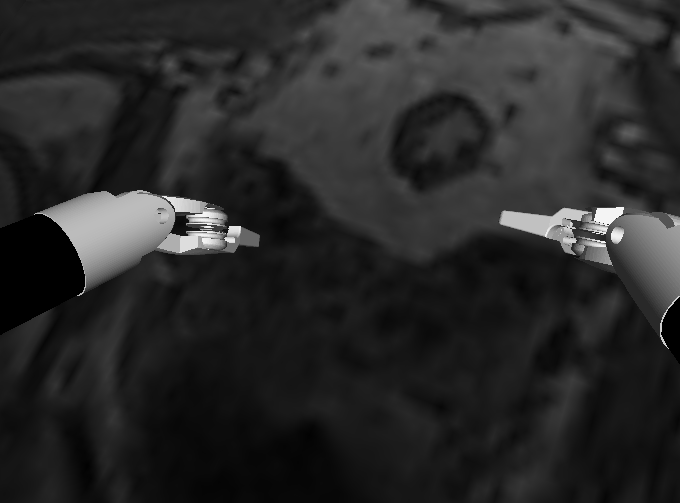
\includegraphics[width=0.6\linewidth]{integration/console_view}
  \caption{View from stereoscopic camera as seen from surgeon’s console.}\label{fig:stereoscopic_console}
\end{figure}

\hrule%

\subsection{Stereoscopic Rendering}\label{ssec:stereo_rendering}

We have implemented true off-axis stereoscopic rendering as shown below where a two tubes are rendered in Red-Cyan Anaglyph 3D.

\begin{figure}
  \centering%
	\frame{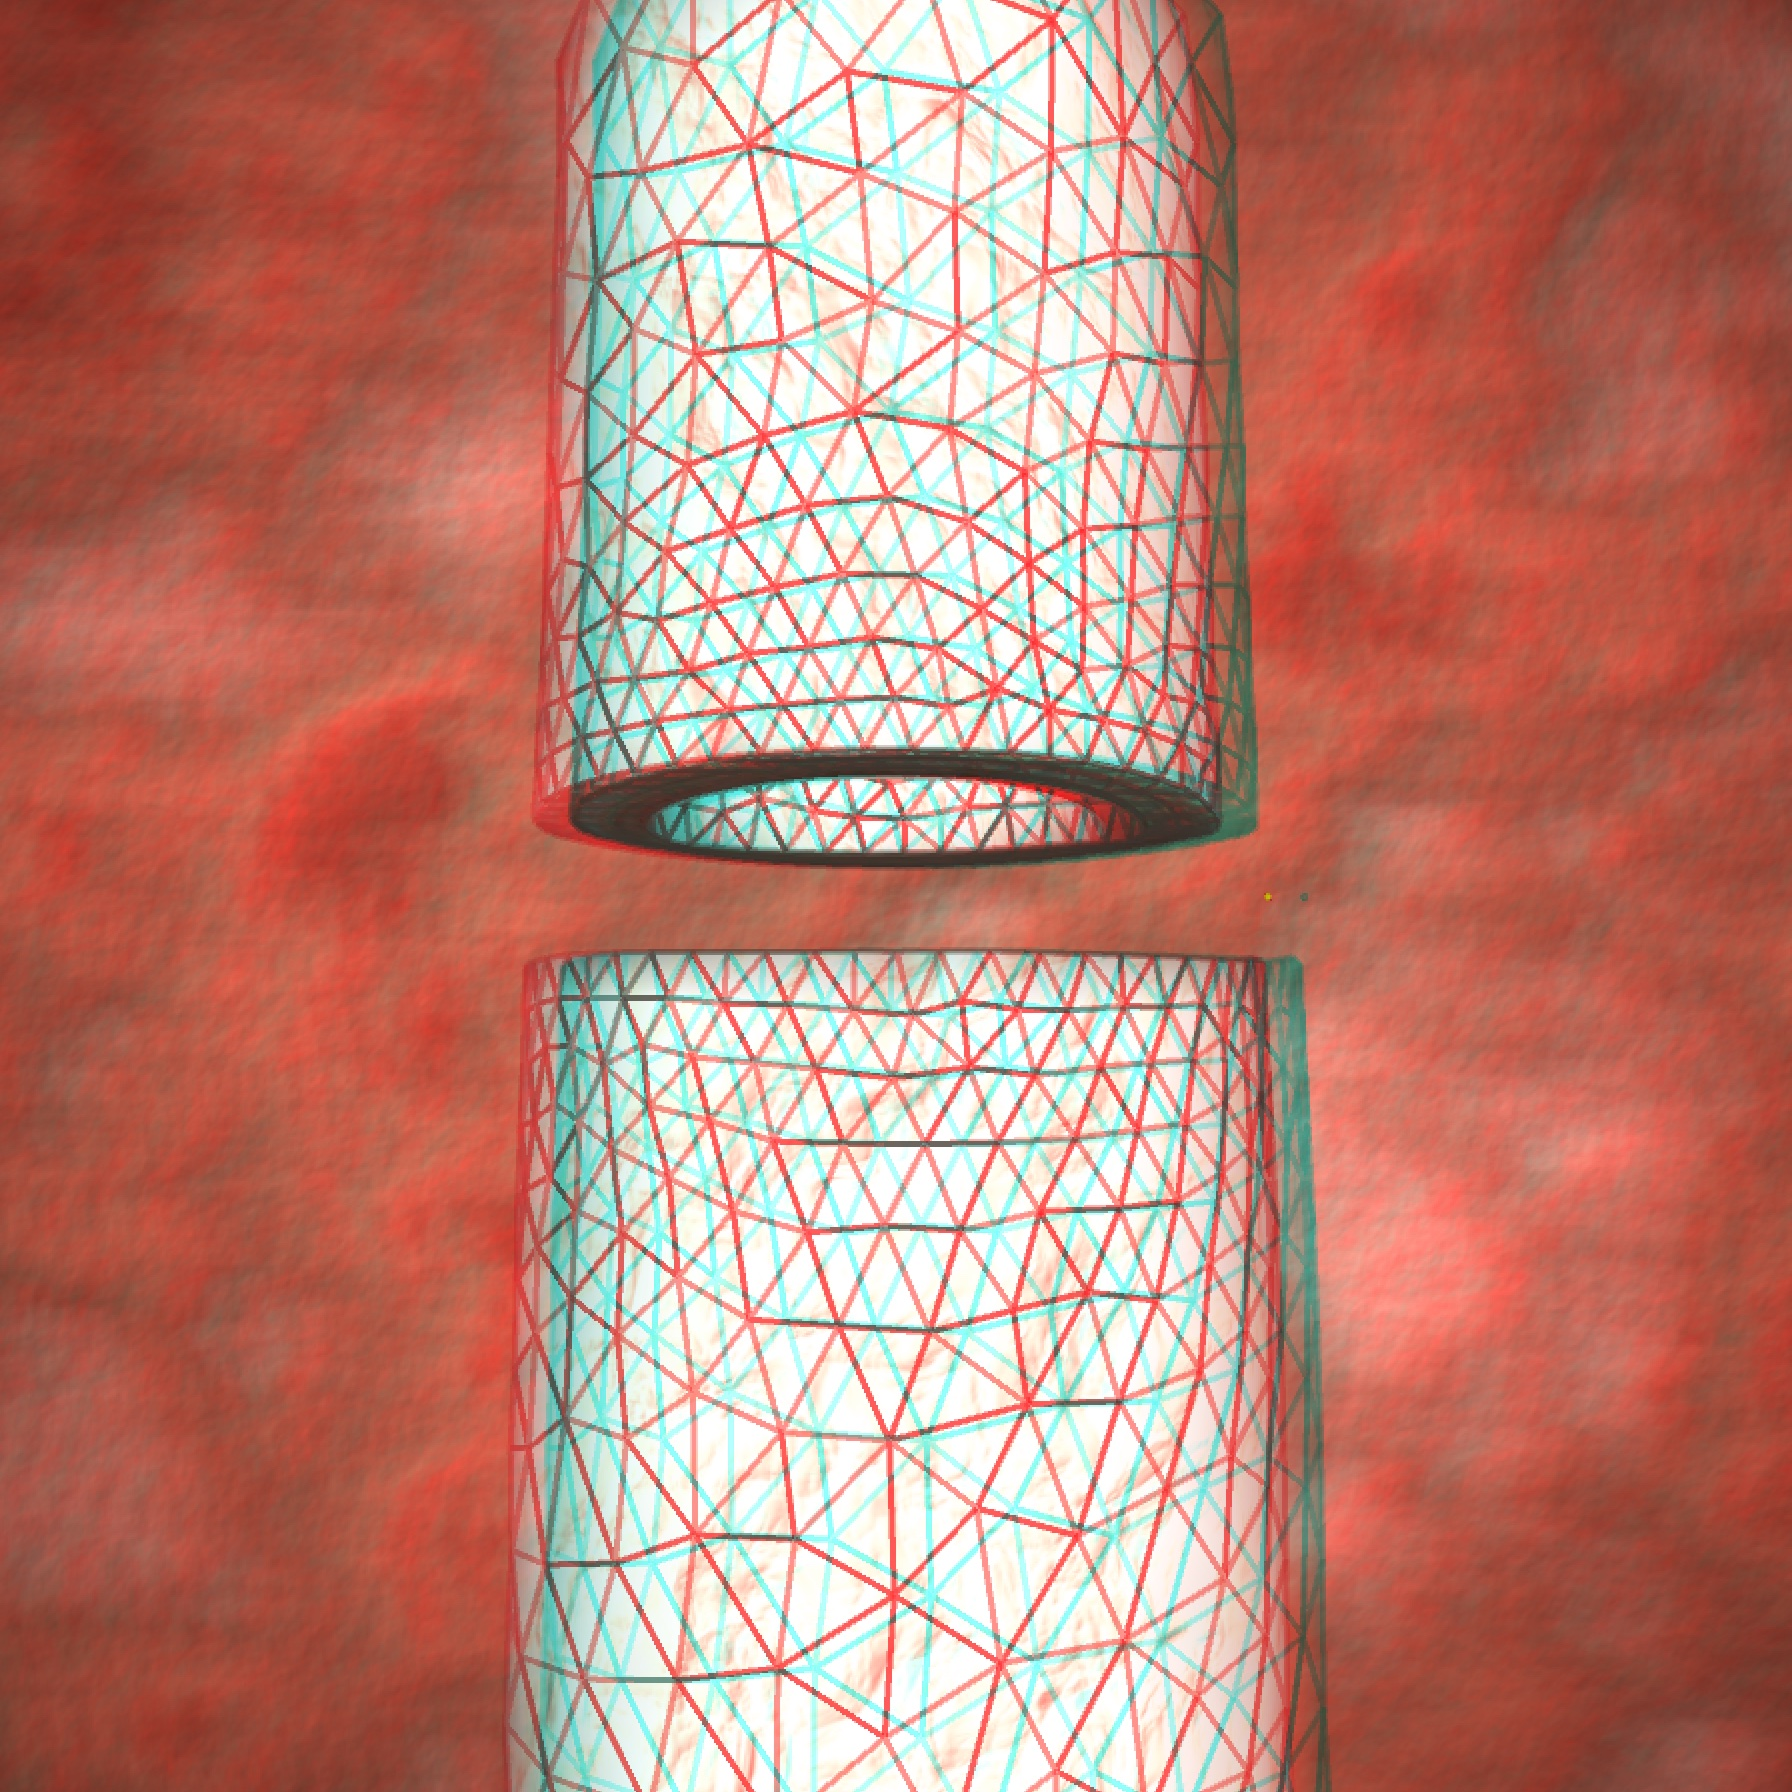
\includegraphics[width=0.5\linewidth]{integration/stereoscopic_anaglyph_red_cyan_rendering}}
	\caption{---}\label{fig:stereo}
\end{figure}

\hrule%

\subsection{Cross-Platform Integration}\label{ssec:cross}
We have created a cross-platform pipeline for continuous integration between our different collaborating teams. Our prototype compiles (using CMake) and runs on all three major platforms: Windows (10 Pro), macOS (High Sierra), and GNU/Linux (Ubuntu Bionic Beaver). We're hosting our private source control repository with \href{https://gitlab.com}{GitLab} to streamline the code access and allow us to experiment with different branches, and are currently working on automating our builds if we were to have more collaborators on board or disseminate our product in the future.

\subsection{User Interface}\label{ssec:console}

We're using robust C++11 libraries and frameworks such as GLFW, GLM, CGAL, Boost, and Eigen, and rendering using OpenGL's Core Profile. We've added support for a bimanual interface using a pair of 3Dconnexion Spaceballs, shown in \autoref{fig:spaceball}, and we're also collecting all the various metrics outlined in Aim 5. This'll allow to replay the procedures as they happened too.

\begin{figure}
  \centering%
  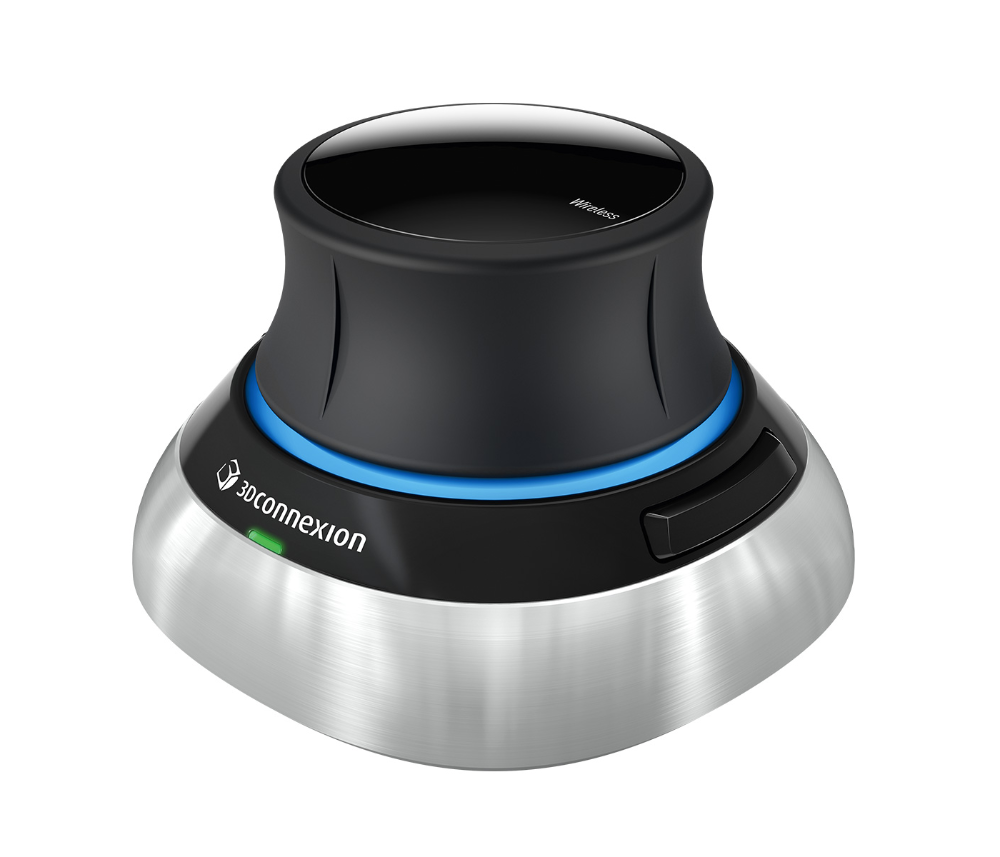
\includegraphics[width=0.32\linewidth]{integration/spaceball_iso_right}
  \hfill%
  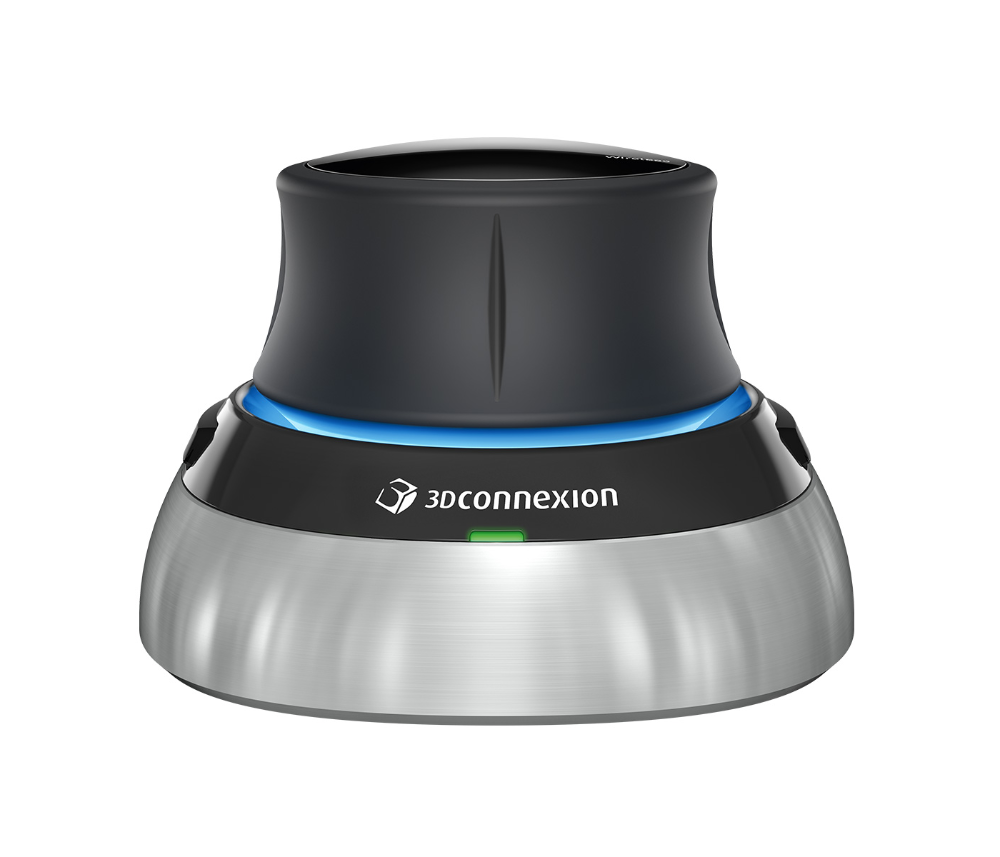
\includegraphics[width=0.32\linewidth]{integration/spaceball_front}
  \hfill%
  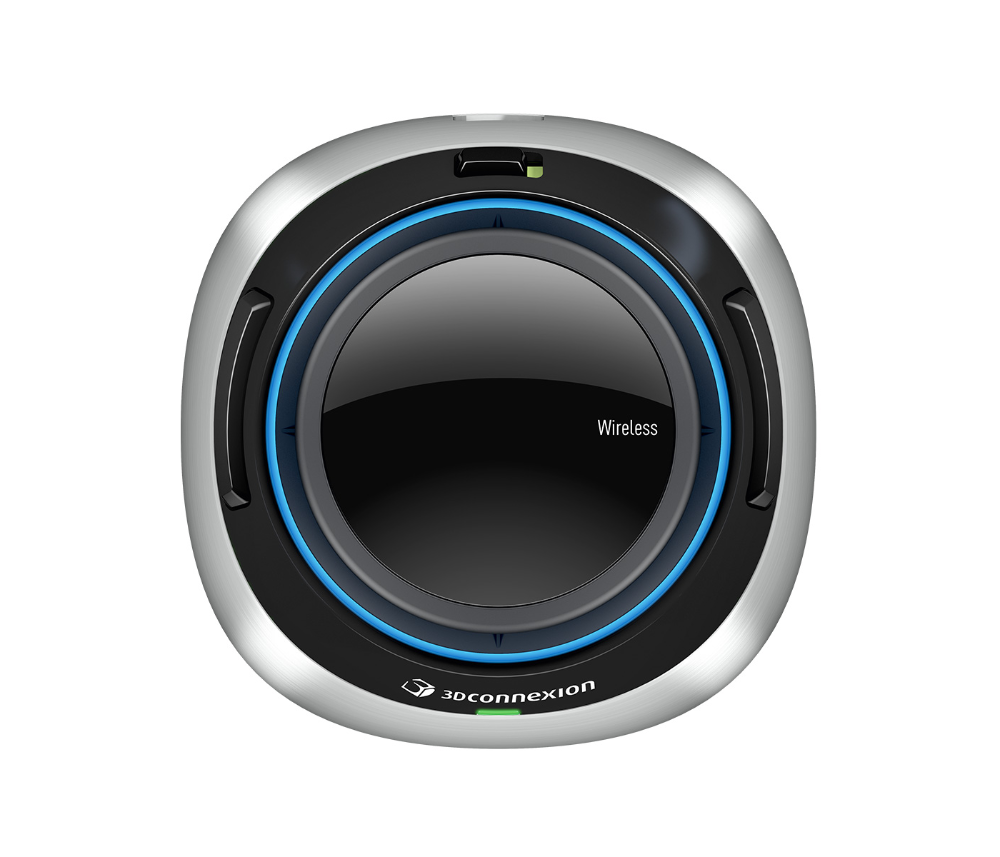
\includegraphics[width=0.32\linewidth]{integration/spaceball_top}
  \caption{Three views of the 3Dconnexion SpaceBall}\label{fig:spaceball}
\end{figure}

\begin{figure}
  \centering%
  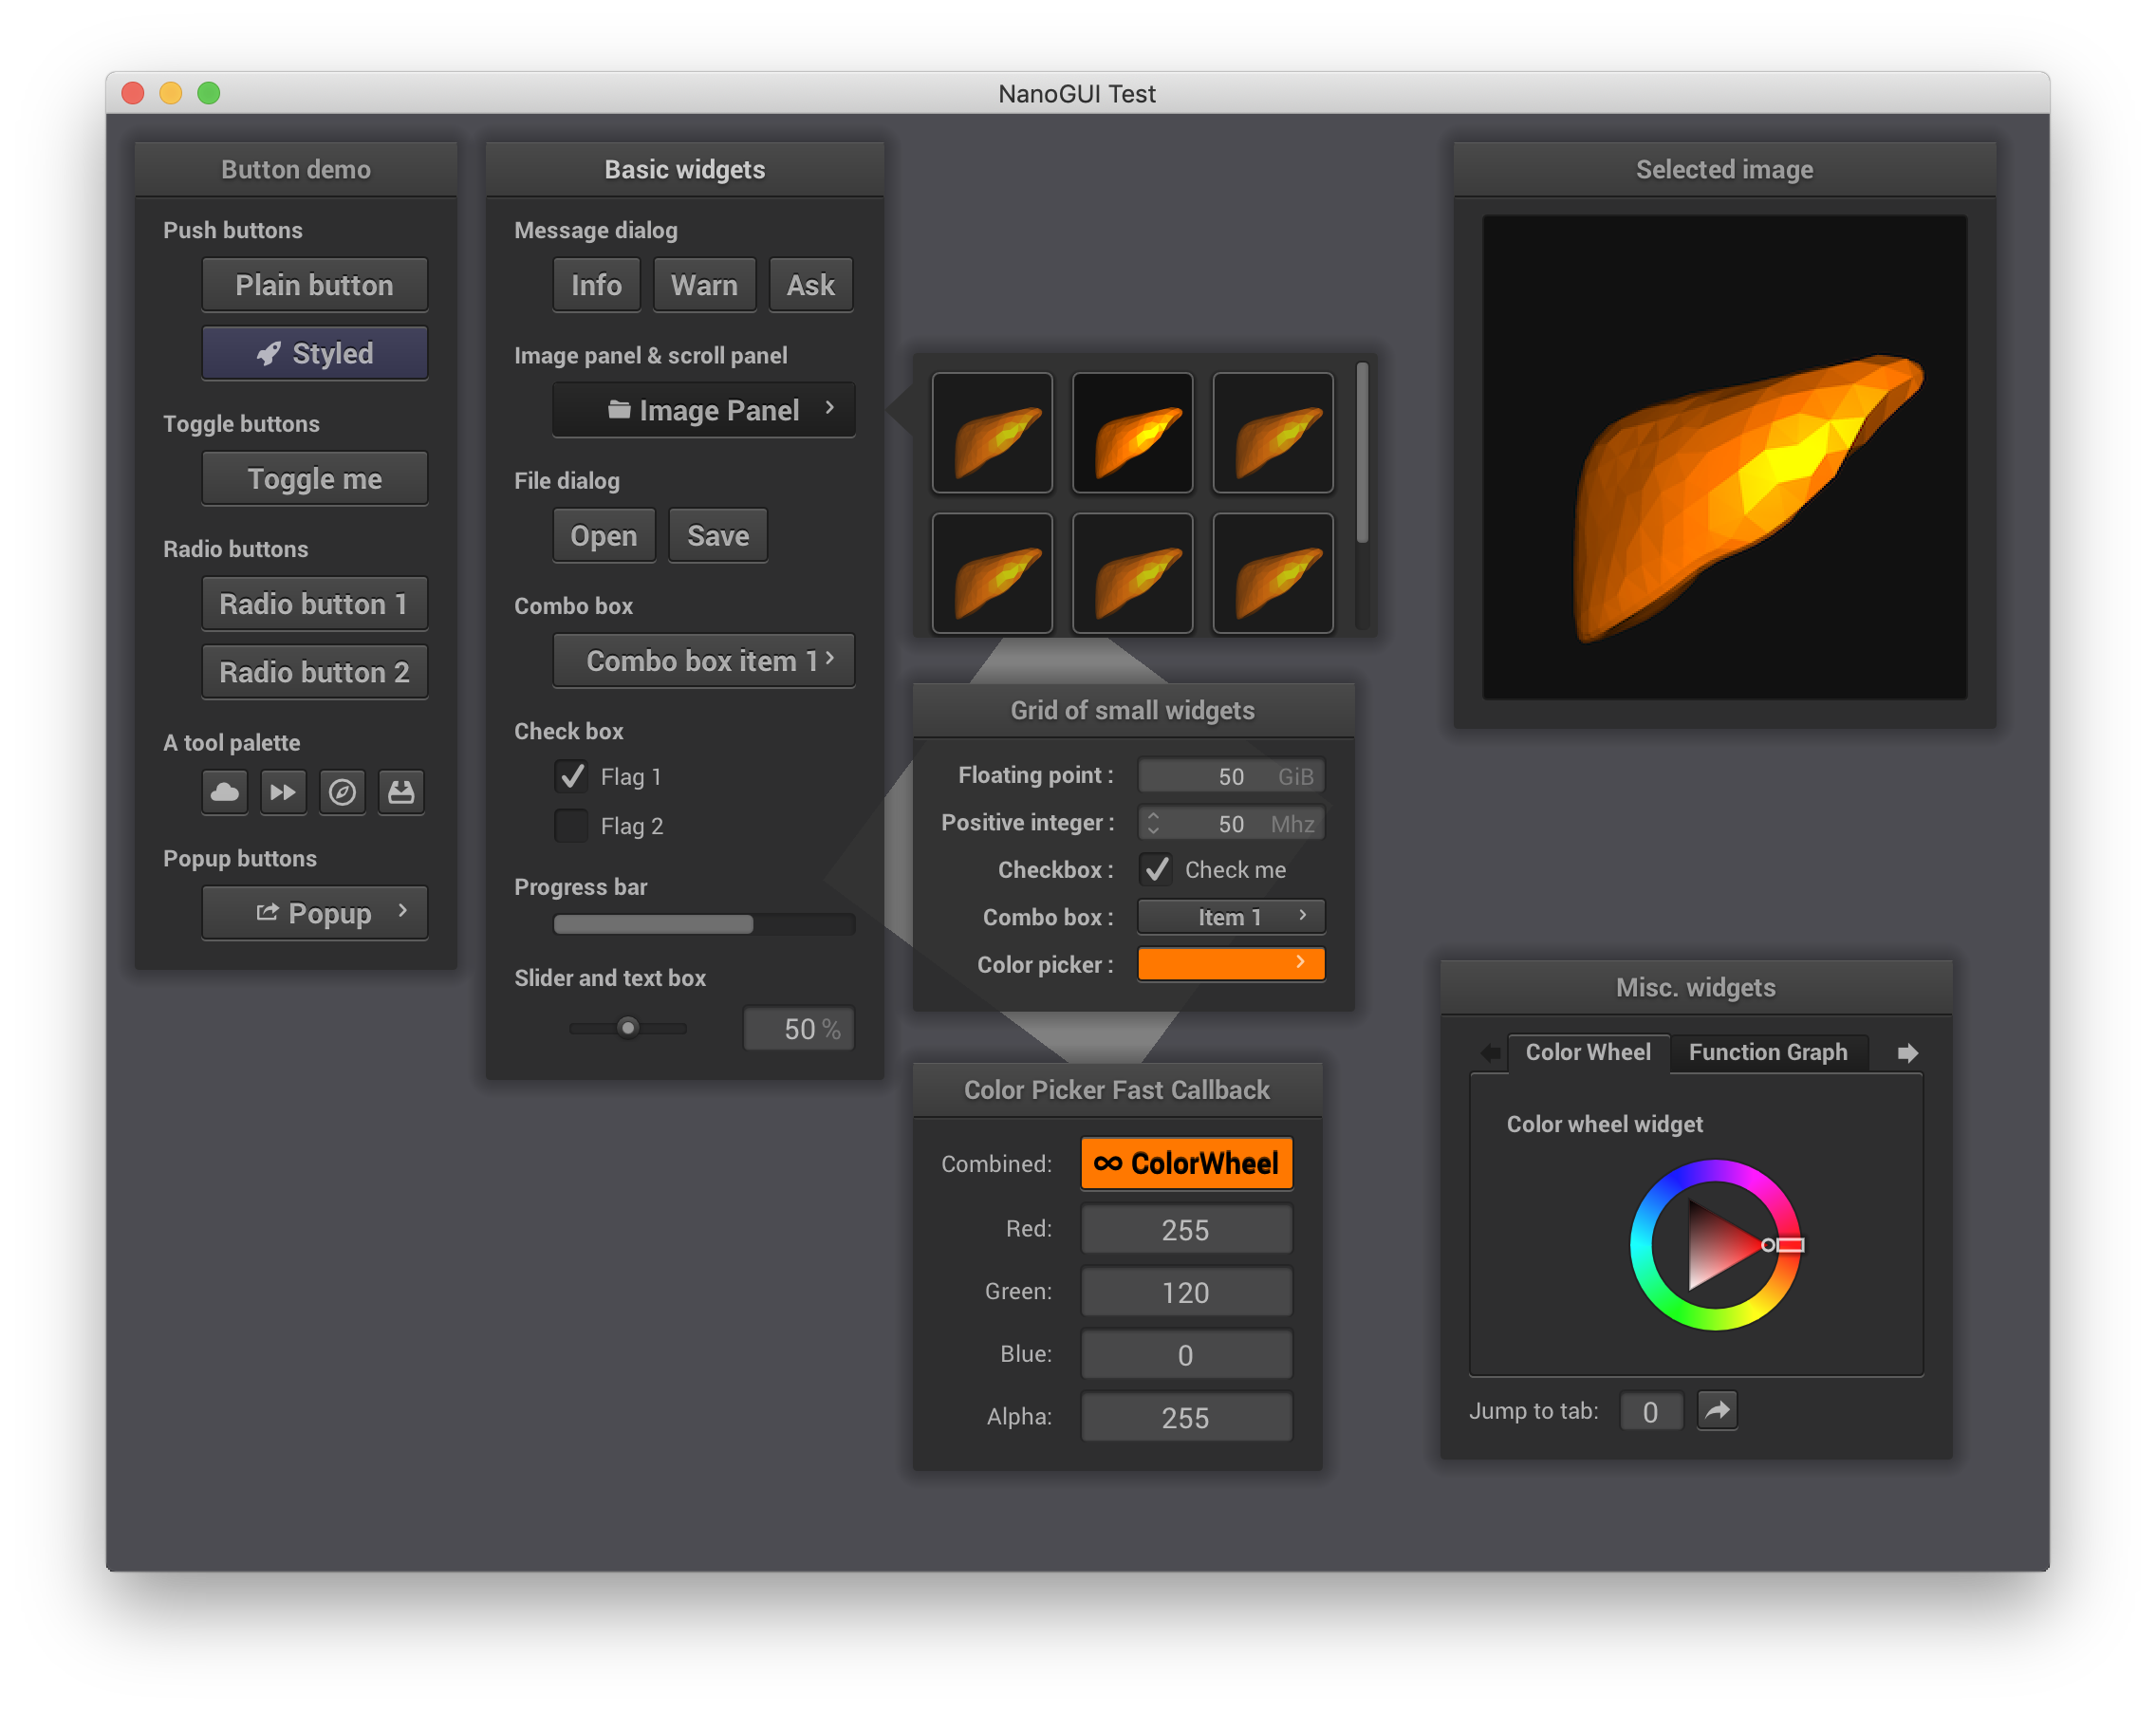
\includegraphics[width=\linewidth]{integration/nanogui_sample}
  \caption{NanoGUI widget library example}\label{fig:nanogui}
\end{figure}

We've added support for Head-up Displays (HUD) using NanoGUI widgets. This'll allow us to display user-friendly notifications and queues, and implement the mockups designed in Aim 5. A sample of the what the library is capable of is shown in \autoref{fig:nanogui}.

An interactive animation from our system integrating the outcomes from the various aims is available at \url{https://www.dropbox.com/s/ax9kmdhaeq91puc/scind_gui.mp4}.

\subsection{Haptic Control}\label{ssec:haptic}
We're using the OpenHaptics framework and the 3D System Touch, shown in \autoref{fig:touch}, to render the forces relayed from the finite element method kernel from Aim 2.

\begin{figure}
  \centering%
  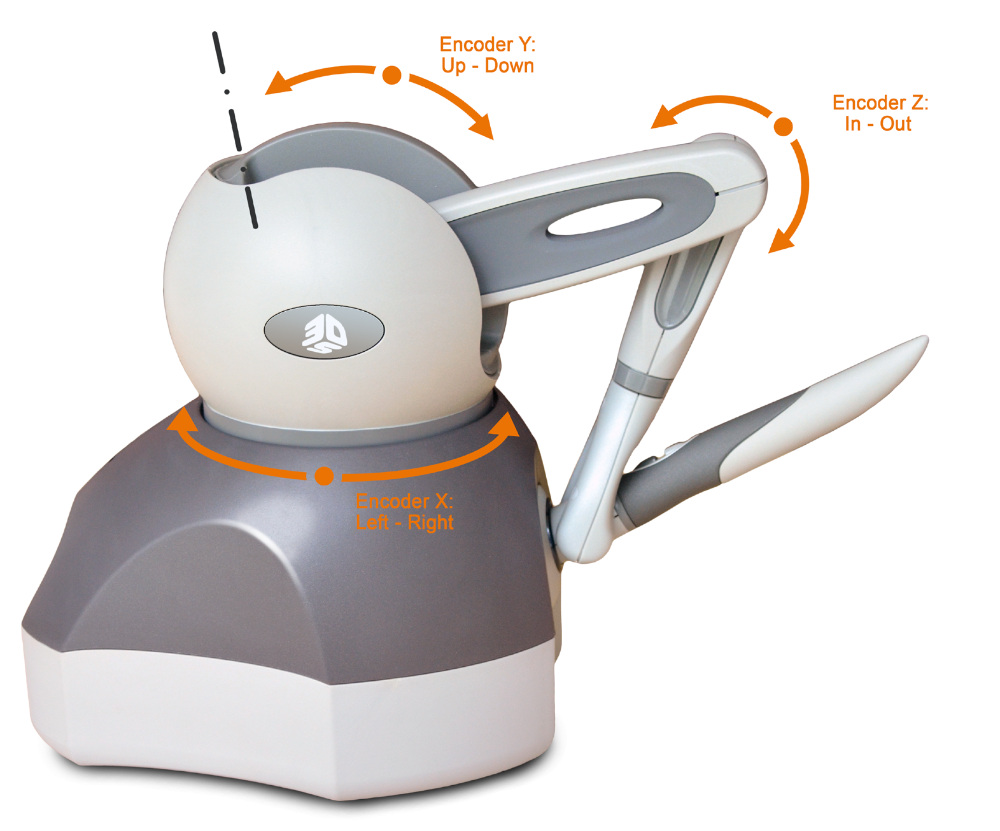
\includegraphics[width=0.48\linewidth]{integration/touch_hero_encoders}
  \hfill%
  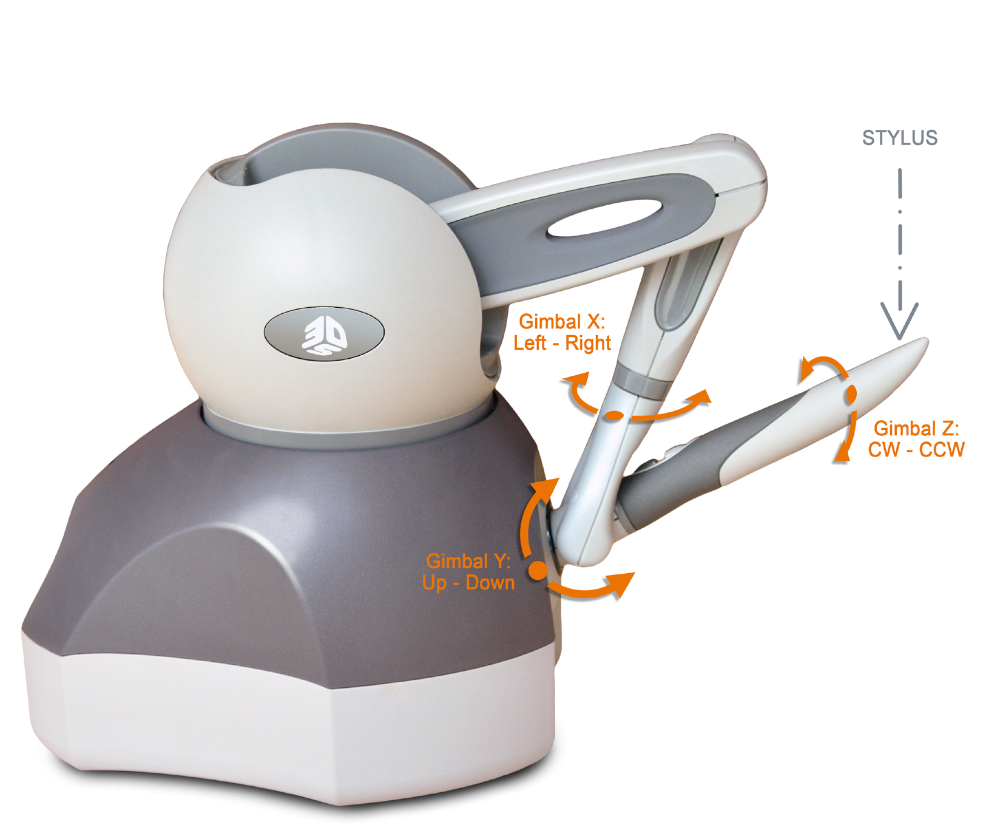
\includegraphics[width=0.48\linewidth]{integration/touch_hero_dofs}
  \caption{Different encoders and degrees of freedom for 3D Systems Touch}\label{fig:touch}
\end{figure}

\subsection{Stereoscopisc Rendering}\label{ssec:stereo}
\begin{figure}
  \centering%
  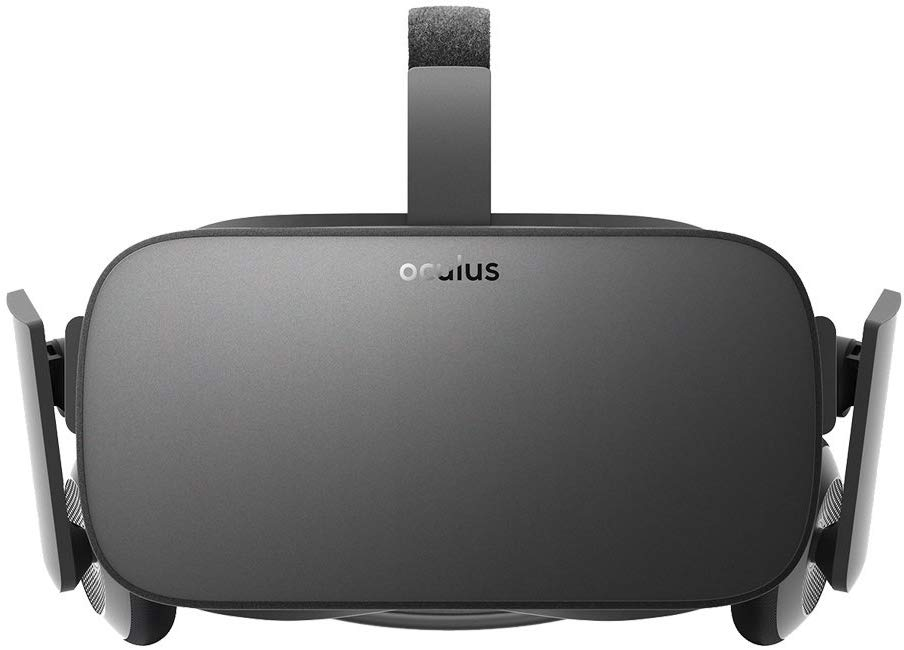
\includegraphics[width=0.45\linewidth]{integration/oculus_rift}
  \hfill%
  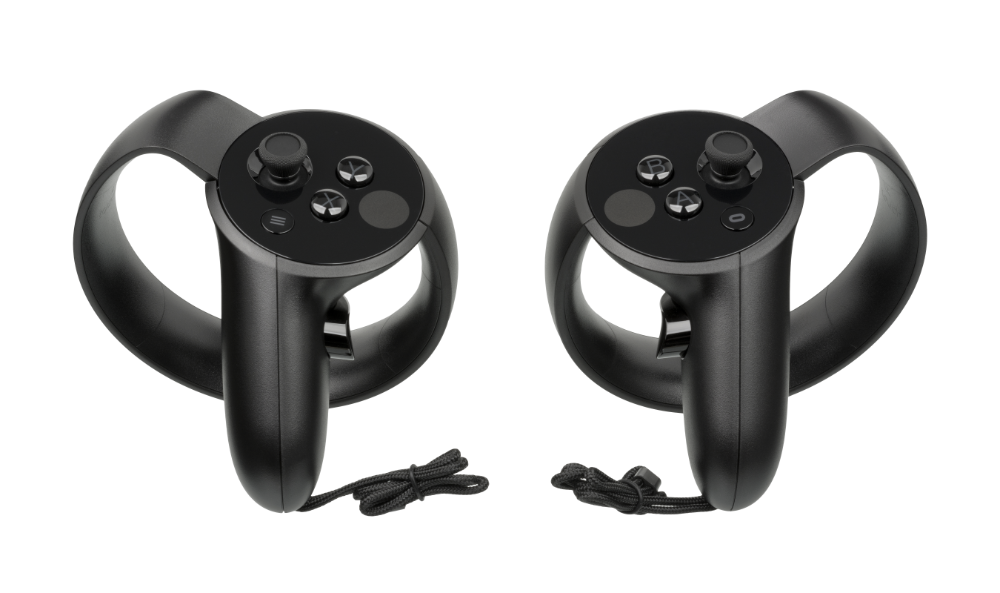
\includegraphics[width=0.54\linewidth]{integration/oculus_rift_touch}
  \caption{Oculus Rift and Oculus Touch}\label{fig:oculus}
\end{figure}

We've enhanced our stereoscopic rendering techniques to work better with stereo displays and we're working on extending our routines to support Oculus Rift and Touch shown in \autoref{fig:oculus} for a more immersive experience.

\hrule%

\begin{enumerate}
  \item Photo from spider interface PR #
  \item EndoWrist kinematics slides PR 2
\end{enumerate}

\hrule%

\section{Cross-Platform Integration}\label{sec:cross}

We have integrated more libraries into our CMake-based build process. Our whole system is now under one repository with centralized access to all collaborators.

\section{User Interface}\label{sec:console}
To simulate a realistic presentation of a medical surgery for surgeons to train on, we need to have the same graphical interface as the real surgeries. Hence we need to mimic the graphical interface of the surgical robot in our simulation, but with the addition of feedback queues to help trainees understand their actions during the surgery.

Using a C++ graphical library that can be layered on top of our simulation, easy to use and has no extra/separate code or libraries required, and that works on all three major operating systems: Windows, macOS, and GNU/Linux). To achieve this we decided to try out two of the most popular and widely used C++ graphical user interface libraries: NanoGUI and ImGUI.

\subsection{NanoGUI}\label{ssec:nanogui}
We went with NanoGUI first to assess it according to our requirements. NanoGUI is a minimalistic cross-platform widget library written in C++ for OpenGL which already meets two of the requirements. We started with testing it with our basic requirements by adding images, buttons, inputs, and drop-down menus. The widgets additions were fairly simple and looked promising for our goal, but all of the widgets were windowed, as can be seen below.

\begin{figure}
  \centering%
  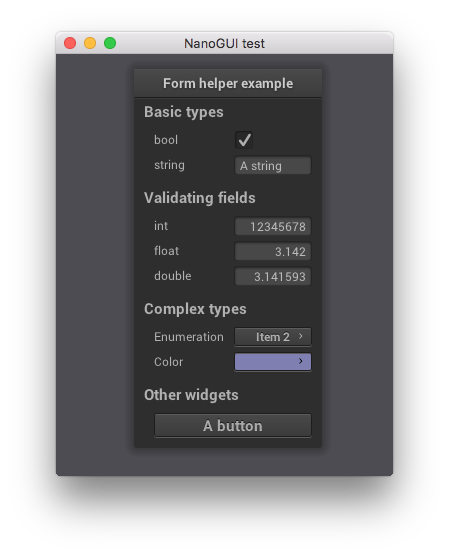
\includegraphics[width=0.5\linewidth]{integration/nanogui}
  \caption{---}\label{fig:}
\end{figure}

Next we went on to see if we can make the widgets translucent, especially images. We were able to control the images translucency, but when it came to the other widgets we faced our first obstacle as it wasn’t as direct as the images. For the buttons to be translucent, we had to change the theme of NanoGUI which means it takes effect on multiple widgets that share similar components and all the buttons will be translucent, which does conflict with our needs but it was not a huge issue, and we could work around it by overlaying the transparent widget over an image that act as a non transparent background color for the widget.

Now we need to meet our last requirement, removing the window and the title menu as seen in the figure above. There were no options in NanoGUI to remove them directly, so we needed to find a way to achieve that behaviour. We started with trying to make the title menu completely transparent but with no luck, and same goes for the background of the window. After multiple attempts we managed to bring the widget to the front of both the window and title menu, then resize them to the widget dimensions to make it the only thing visible, as can be seen below with one button. This worked for buttons, text, and inputs, but not for drop-down menus and images. For drop-down menus when clicked on, the dropdown does not show because of the size of the window, while for images, when we make them translucent, the window and title menu show, which is a deal breaker as it violates two of the crucial requirements.

\begin{figure}
  \centering%
  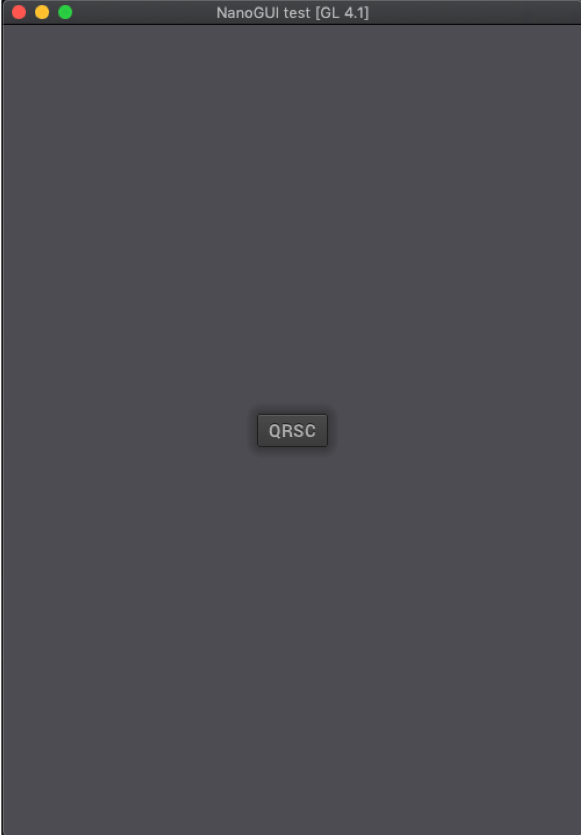
\includegraphics[width=0.4\linewidth]{integration/cropped_button}
  \caption{---}\label{fig:}
\end{figure}

In conclusion, given the behaviour of NanoGUI and the requirements it both met and did not meet, and in addition to the complexity of overcoming some constraints, we marked NanoGUI as an unsuitable tool for this project and other future projects.

\subsection{ImGUI}\label{ssec:imgui}
After deciding on NanoGUI not being a good fit, we moved on to our second option ImGUI. ImGUI is a light-weight graphical user interface library for C++ that is fast, portable, renderer agnostic, and self-contained (no external dependencies). So just like NanoGUI, ImGUI is both written in C++ and cross-platform making it easier for us to integrate it with our simulator. We first started testing ImGUI with removing the window and the title menu, and we managed to do that with only two lines of code, which was a big improvement from NanoGUI both in simplicity and functionality, in addition to controlling the resizing and the movability of the window. After it, we added widgets which had a better structure in the form adding them to our GUI, where each widget such as buttons and labels had their own styling properties that can be applied. In addition, we were able to add images, make them translucent and overlay text on top of them as shown below. Given that, ImGUI met all our requirements, this gave us the green light to go ahead and use it for our graphical interface.

\begin{figure}
  \centering%
  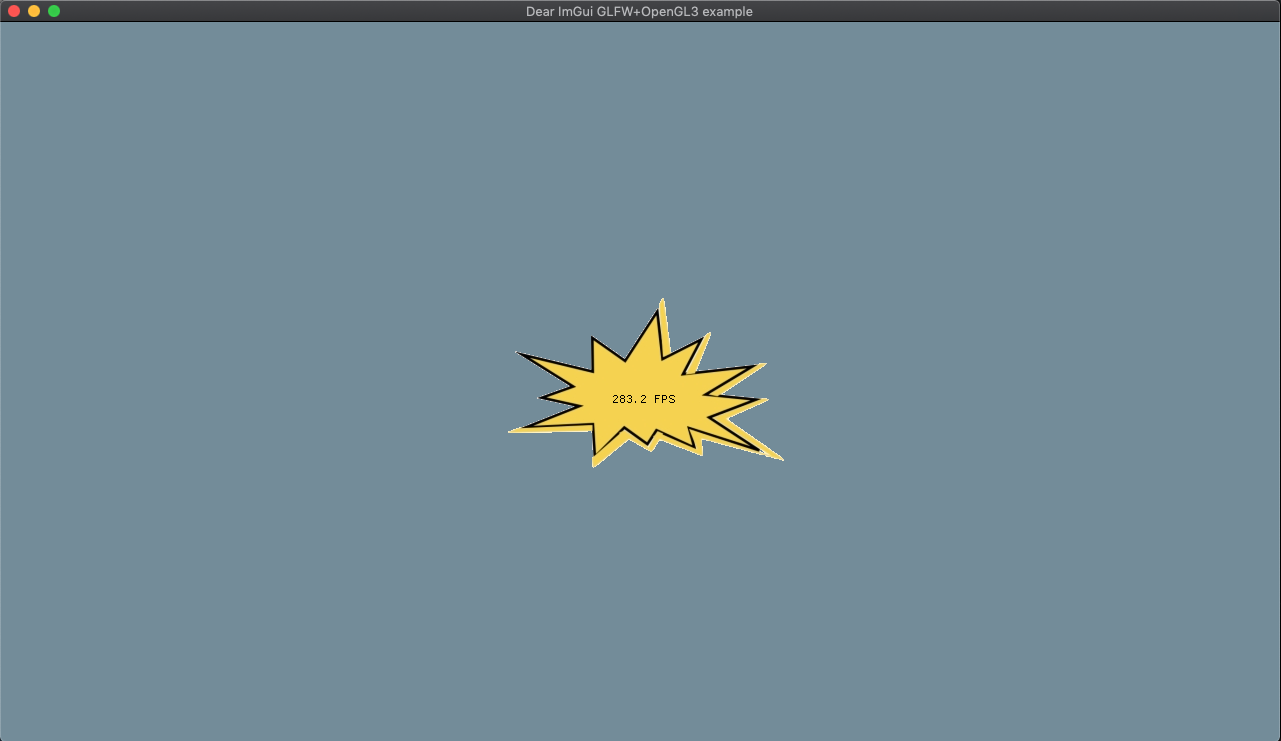
\includegraphics[width=\linewidth]{integration/imgui}
  \caption{---}\label{fig:}
\end{figure}

\subsection{Graphical User Interface}\label{ssec:gui}
We started creating our GUI by looking at the GUI of the da Vinci Robot that is used in the surgeries we are working on simulating for surgeons to train on.

Given these images, we started recreating the widgets in sketch to have them in high resolution to look crisp on all sizes of monitors. In addition, we used our own fonts for the text to give an elegant and simple design to the GUI, especially in the feedback dialogs for the trainees, making it easy for them to read and gentle on their eyes.

\begin{figure}
  \centering%
  \setlength{\fboxsep}{0pt}%
  \setlength{\fboxrule}{0.1pt}%
  \fbox{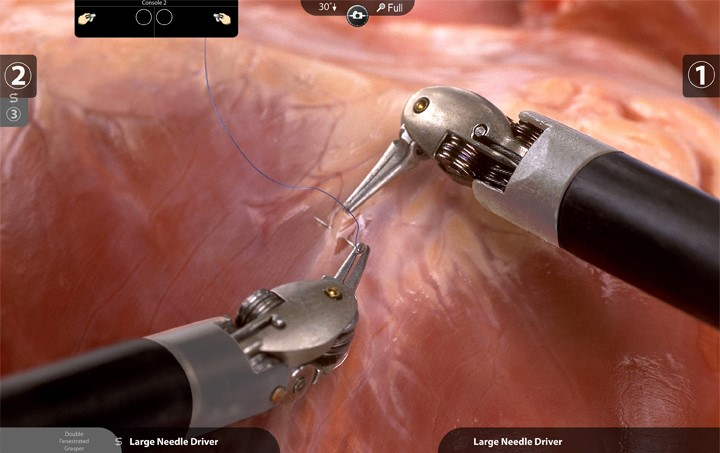
\includegraphics[width=\linewidth]{integration/davinci_snapshot}}\\[1ex]
  \fbox{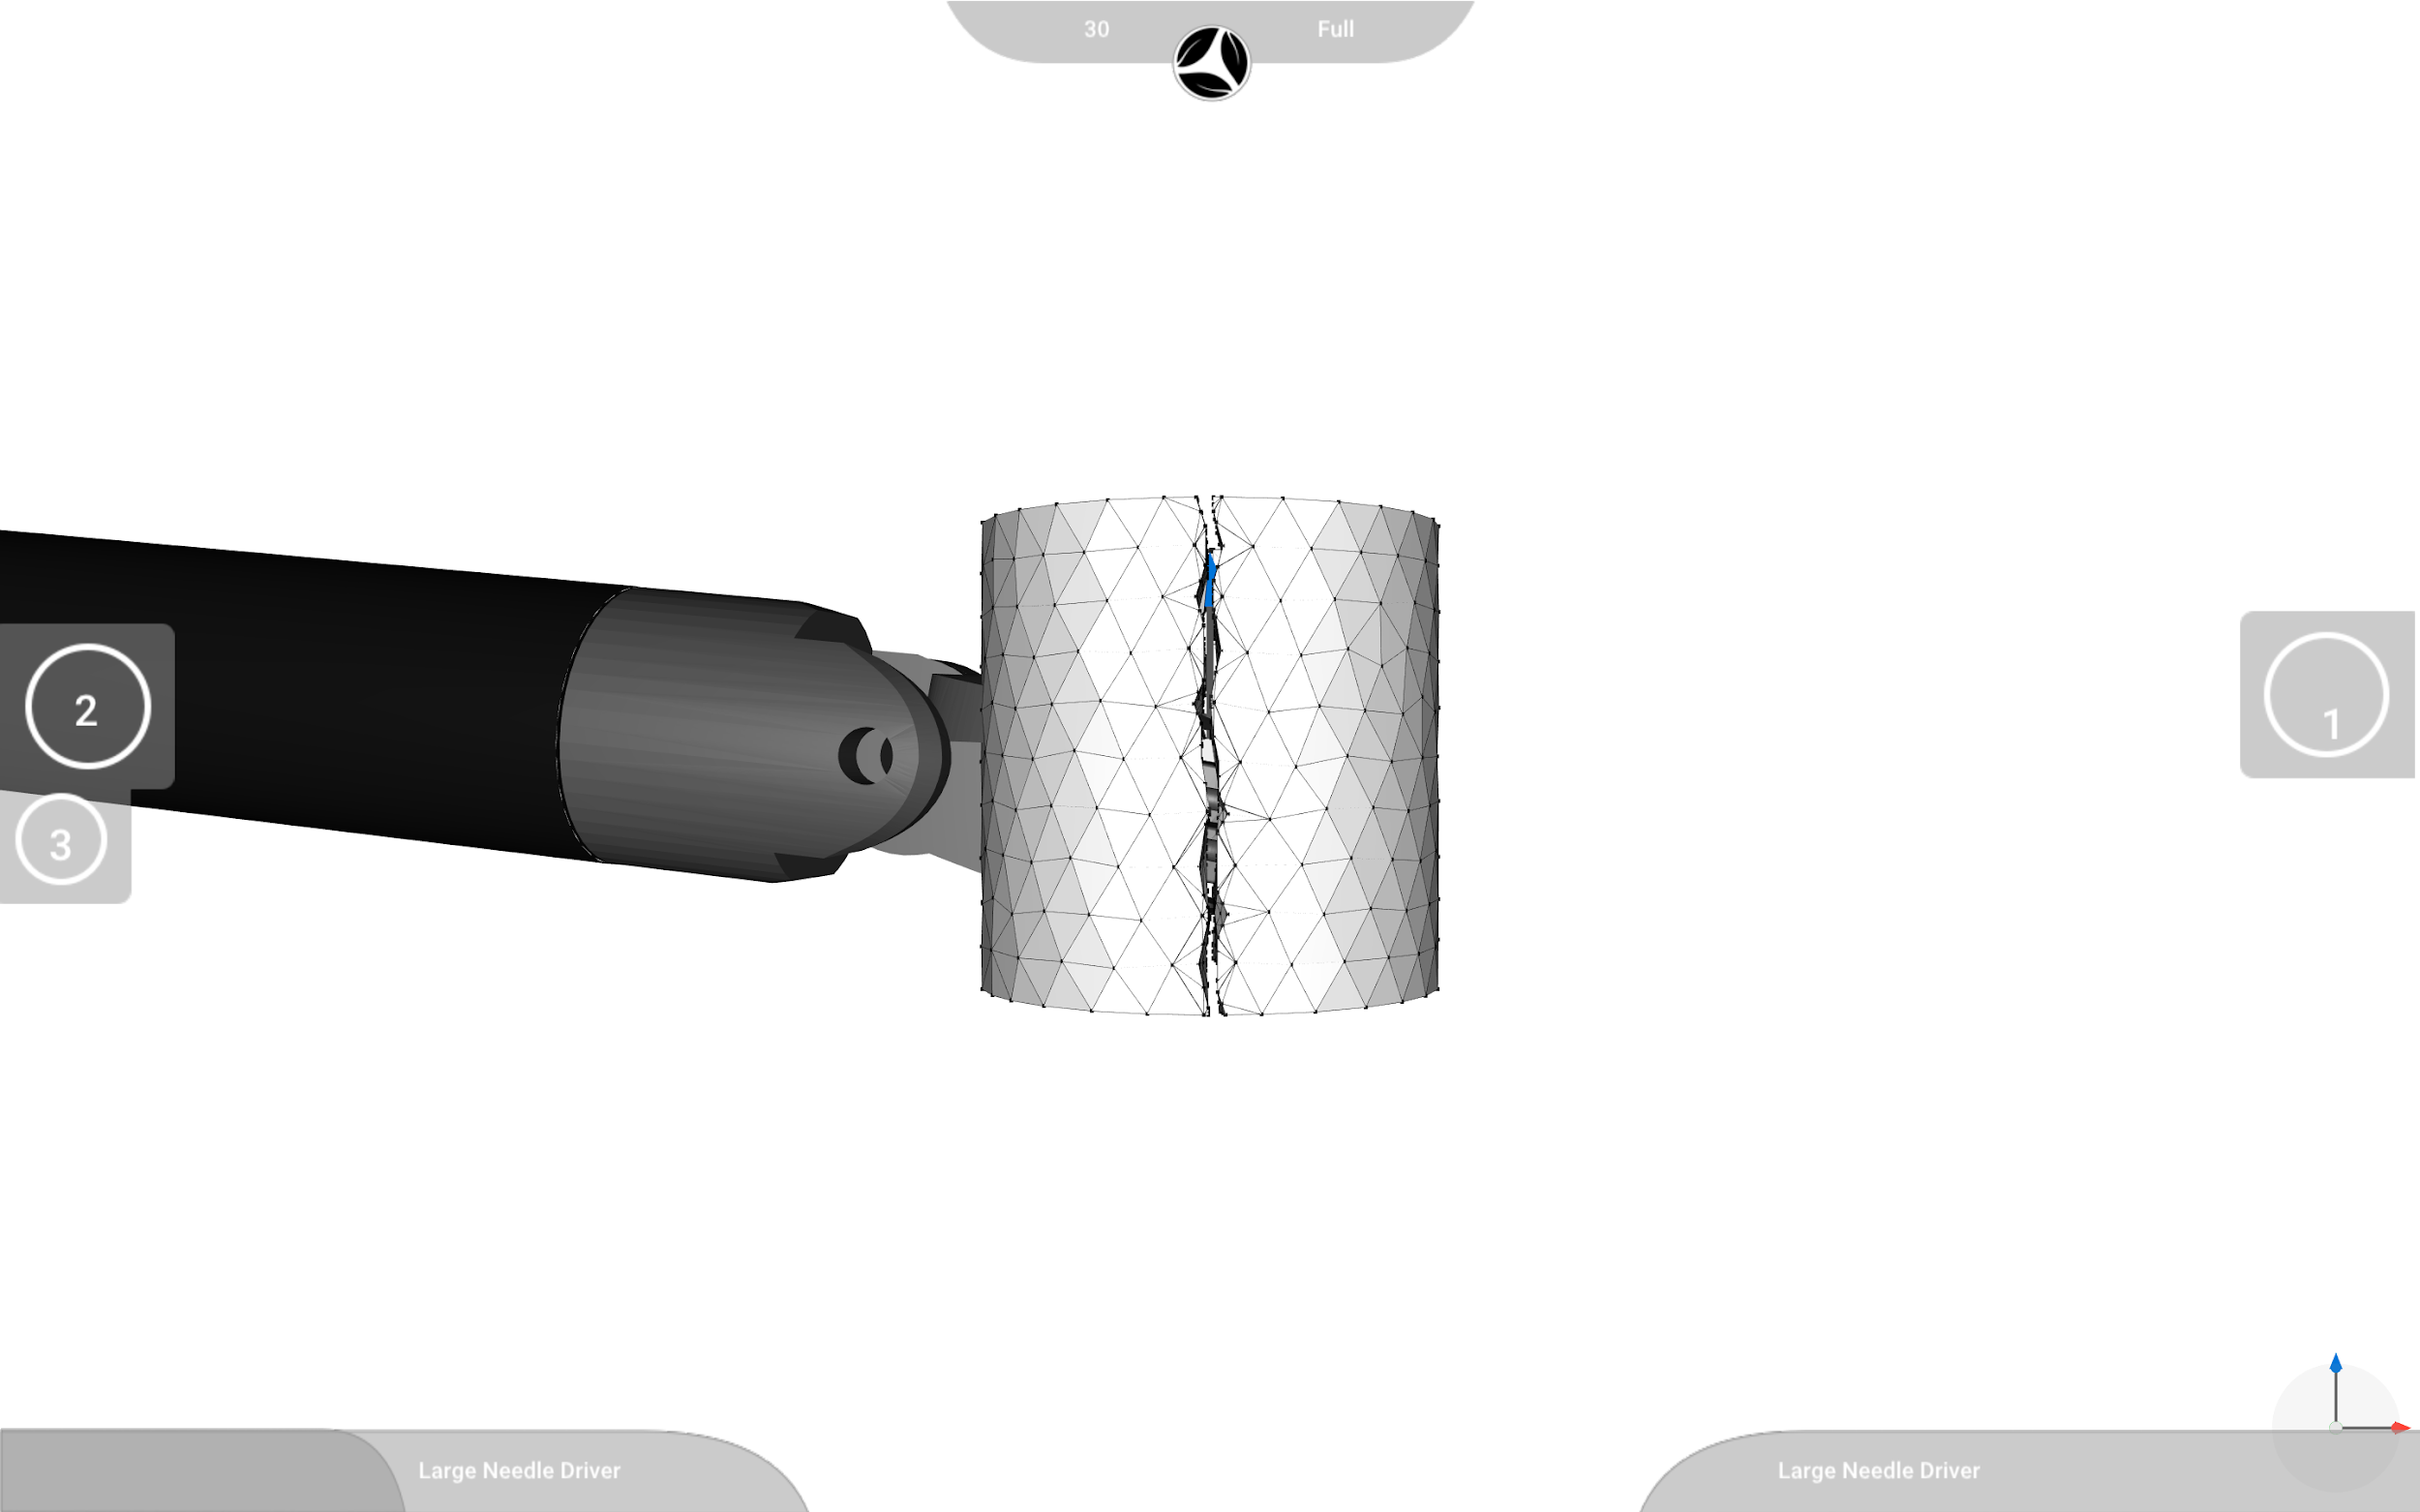
\includegraphics[width=\linewidth]{integration/interface_basic_scind}}
  \caption{---}\label{fig:}
\end{figure}

Following this we decided to add a popup window that allows the user to specify options and settings of the scene, in addition to adding a file dialog window, that in the future would give the user the ability to add their own scenes or models to the simulation.

\begin{figure}
\centering%
\setlength{\fboxsep}{0pt}%
\setlength{\fboxrule}{0.1pt}%
\fbox{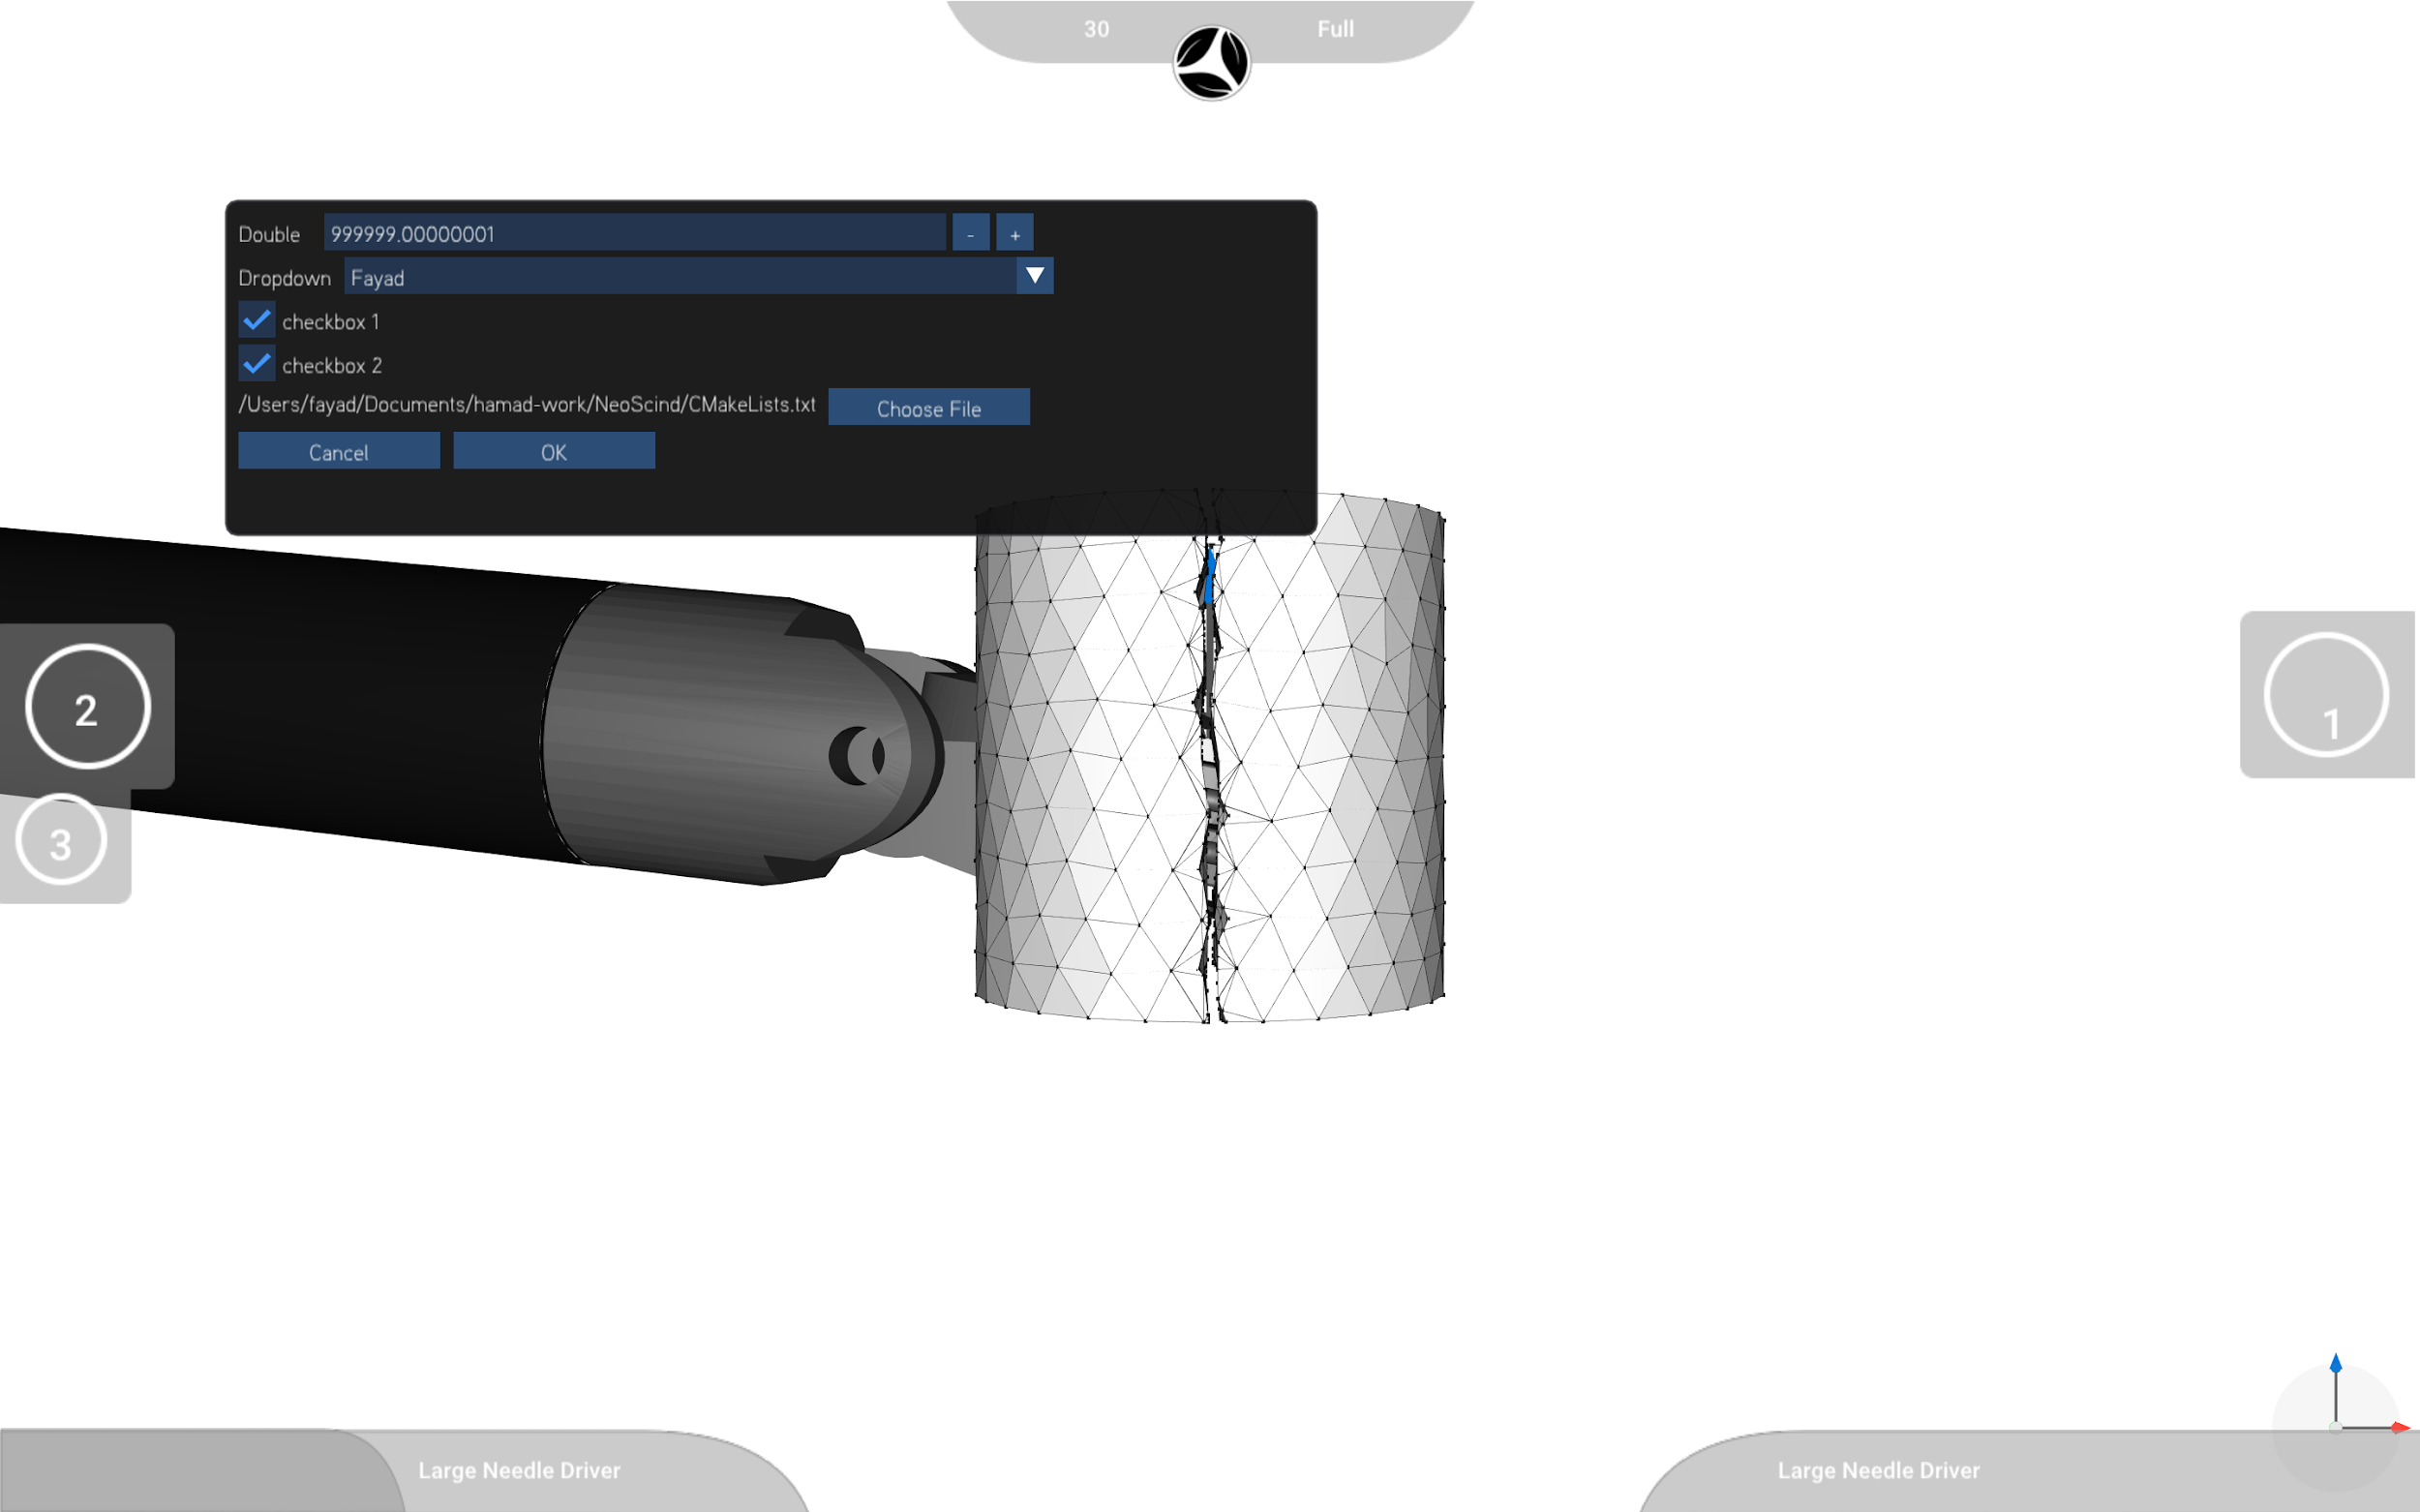
\includegraphics[width=\linewidth]{integration/interface_basic_scind_popup}}
\end{figure}

Finally, we changed the GUI to match the newest da Vinci robot (da Vinci Xi) with the addition of feedback dialogs. The purpose of this is to replicate the feel of real surgeries, so there is a smooth transition when the trainees transition from our simulator to the da Vinci Xi, in addition to giving them feedback on their progress to reinforce learning the right techniques, by giving them a good explanation of why their actions were not ideal in that scenario and the way to correct them.

\begin{center}
  \setlength{\fboxsep}{0pt}%
  \setlength{\fboxrule}{0.1pt}%
  \fbox{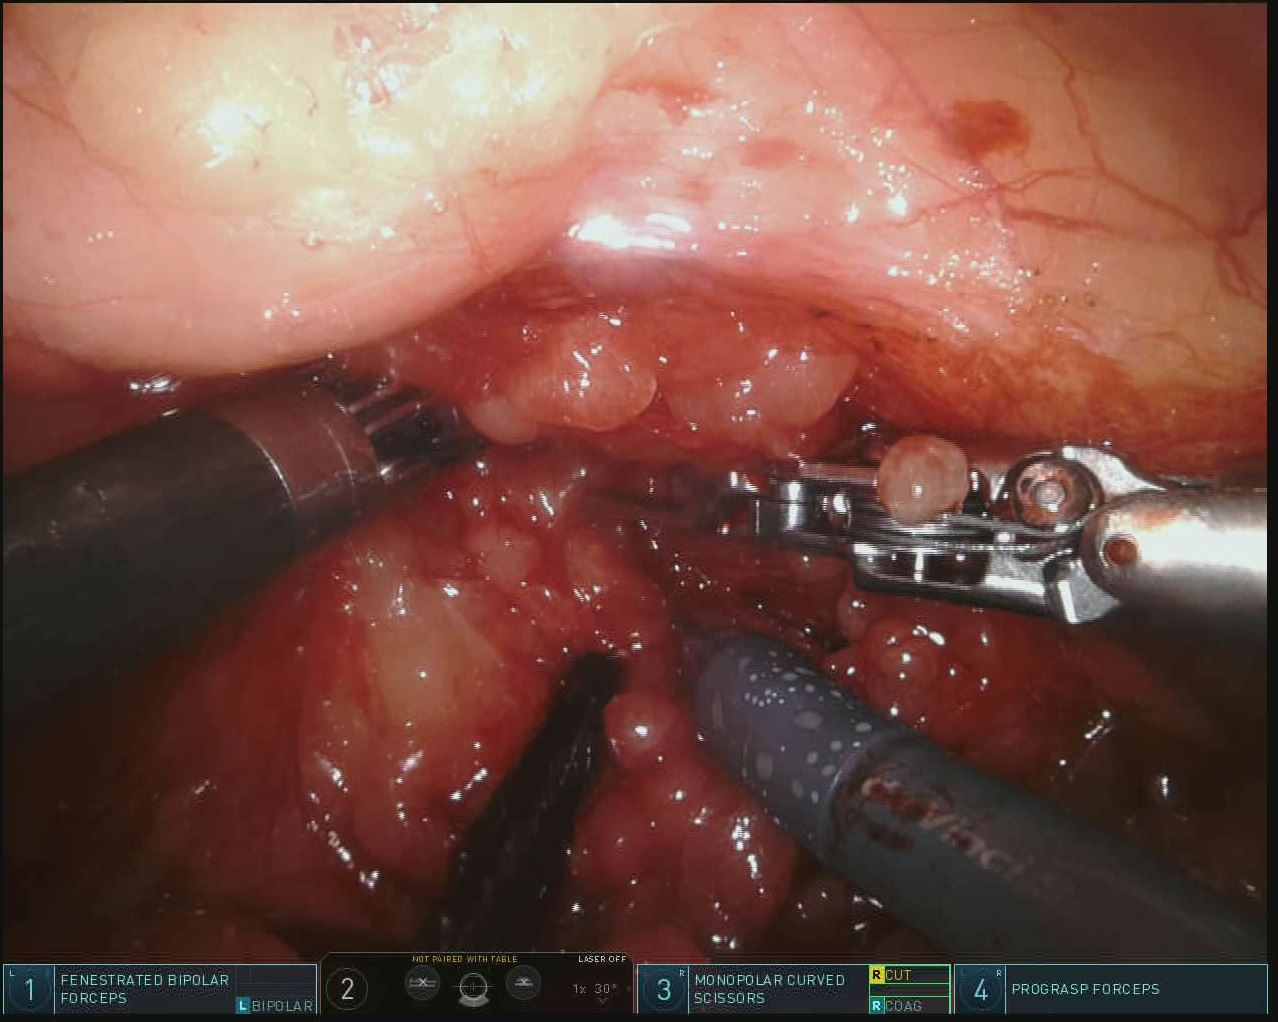
\includegraphics[width=\linewidth]{integration/davinci_xi}}
\end{center}

In conclusion, NanoGUI appeared to be less flexible than ImGUI, giving ImGUI the advantage for us to use it in this project and future projects. Furthermore, we managed to recreate the da Vinci robot GUI to have a simulation that resembles the real feel of surgeries as much as possible, at least when it comes to the graphical interface.

\begin{figure}
  \centering%
  \setlength{\fboxsep}{0pt}%
  \setlength{\fboxrule}{0.1pt}%
  \fbox{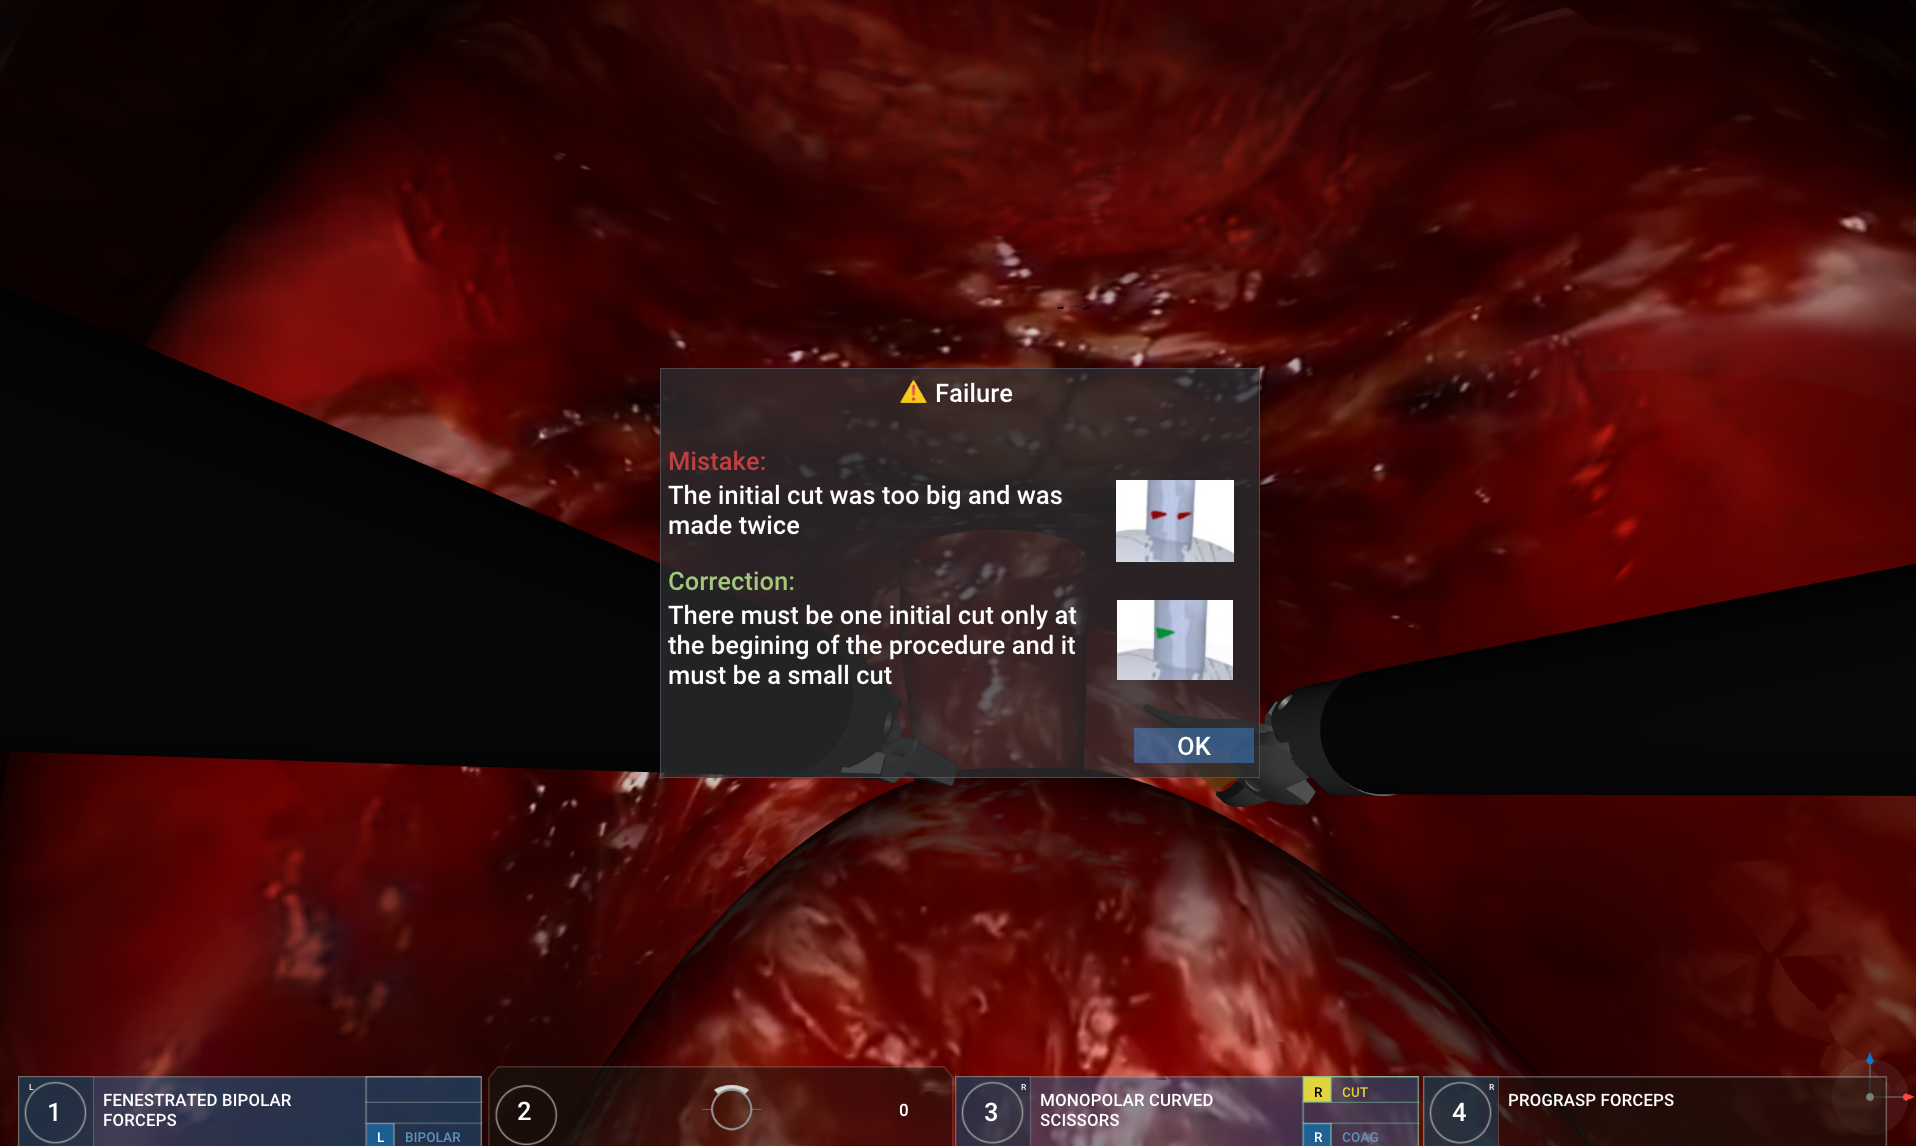
\includegraphics[width=\linewidth]{integration/interface_scind}}\\[1ex]
  \fbox{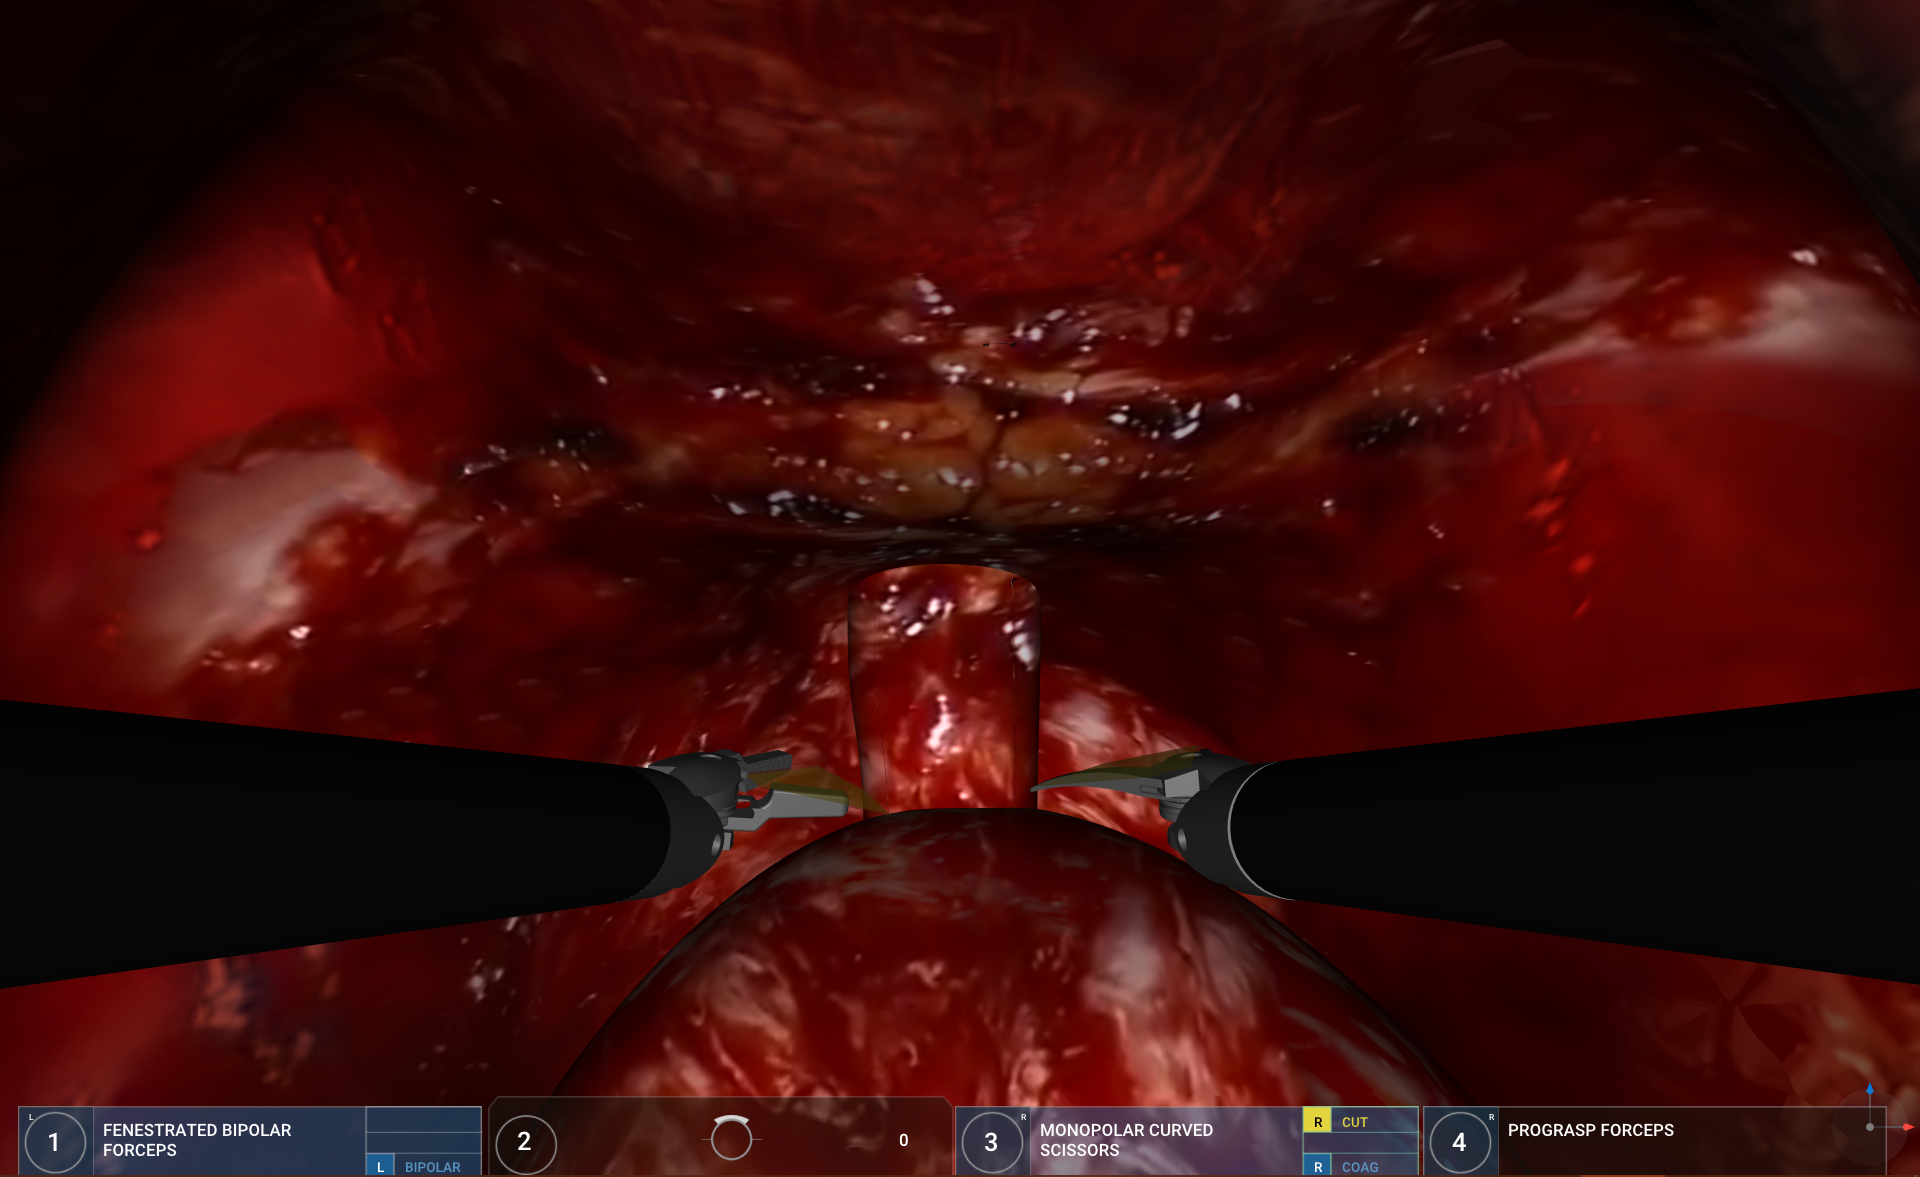
\includegraphics[width=\linewidth]{integration/interface_scind_popup}}
  \caption{---}\label{fig:}
\end{figure}

%\section{Haptic Control}\label{sec:haptic}

%\section{Stereoscopic Rendering}\label{sec:stereo}

\section{SOFA}\label{sec:sofa}
We want to create a robotic surgery simulator similar to what we are making but in using the available solutions that exist to have a comparison to evaluate and measure our solution performance to them.

Using SOFA framework as a tool to develop the robotic surgery simulation. SOFA is an efficient framework dedicated to research, prototyping and development of physics-based simulations that is both open source and cross-platform, this gives the ability to use it freely and modify it on the same three platforms we work on. We wanted to use SOFA since it is extensively used in medical simulation and is mature enough for development since it is been around since 2005.

We want to do the following tasks in SOFA:
\begin{enumerate}[1.]
  \item Loading of both surface and volumetric 3D models (VTK, OBJ, STL, and other),
  \item Deformation of 3D models,
  \item Cutting of 3D models, and
  \item Using the omni phantom as a user input interface.
\end{enumerate}

\subsection{Loading 3D models}
We want to be able to load 3D models to apply the other functions we need. Loading both volumetric and surface 3D models in SOFA was fairly straightforward. Next step, was adding textures to these models, and rendering them was a built-in function.

\begin{figure}
  \centering%
  \setlength{\fboxsep}{0pt}%
  \setlength{\fboxrule}{0.1pt}%
  \fbox{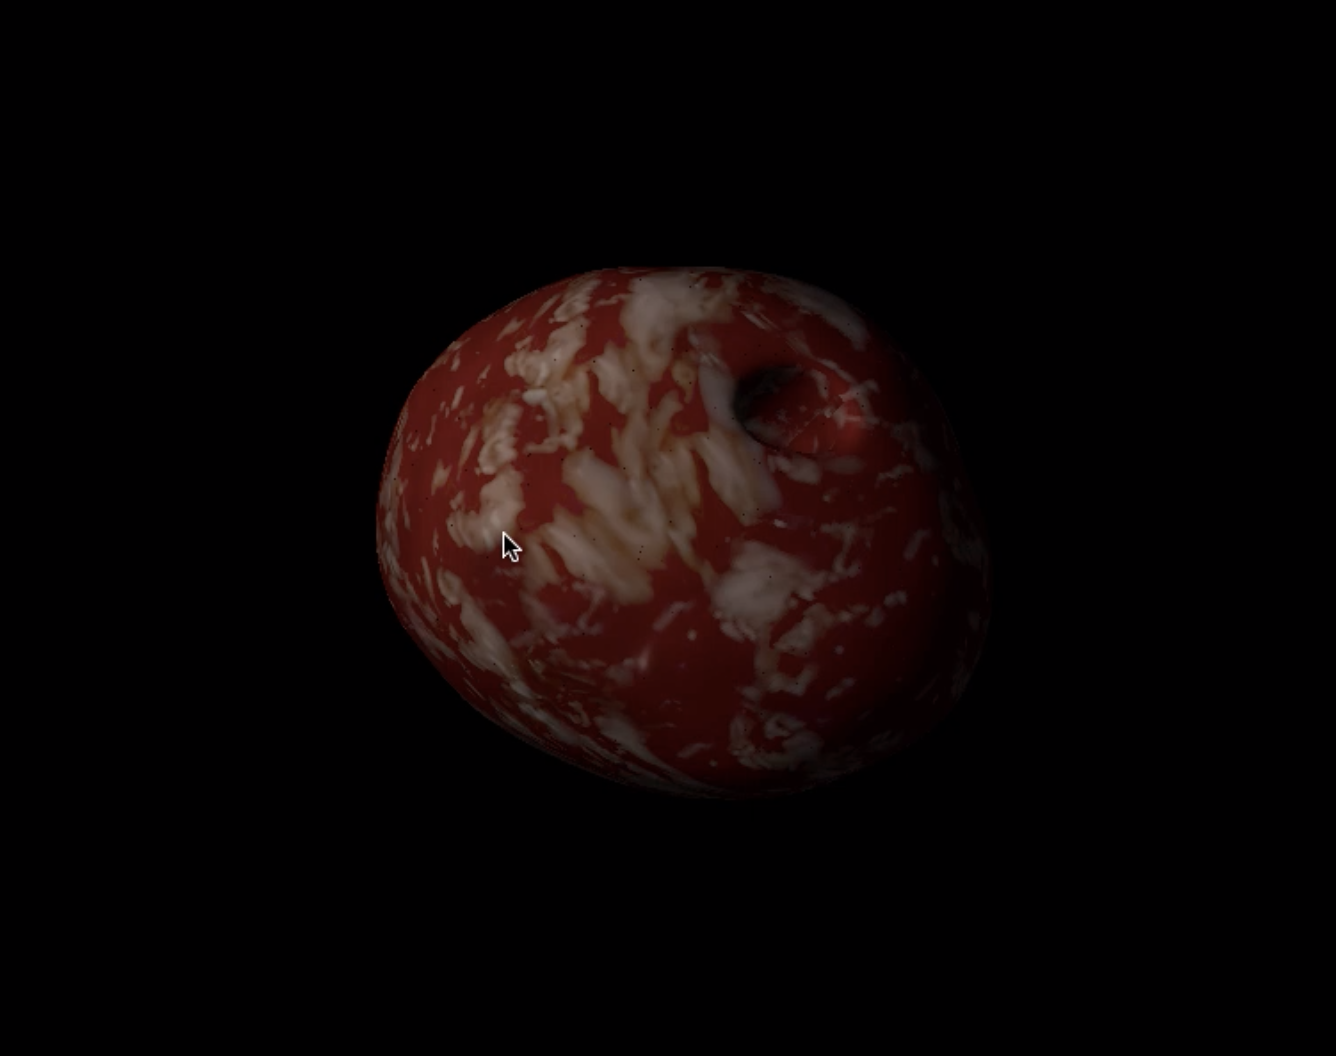
\includegraphics[width=0.7\linewidth]{integration/sofa_textures}}
  \caption{---}\label{fig:sofa_textures}
\end{figure}

\subsection{Deformation}
Next step was us looking at the physics of the engine, specifically the deformation. SOFA provided multiple types for the model to take, Rigid, Vec3, Vec6. The Vec3 type give us the deformable behaviour we want, which is added to the model in the loading part by changing the template. In addition, we used the rigid body template for the scissors as they need not to deform on impact.

\begin{figure}
  \centering%
  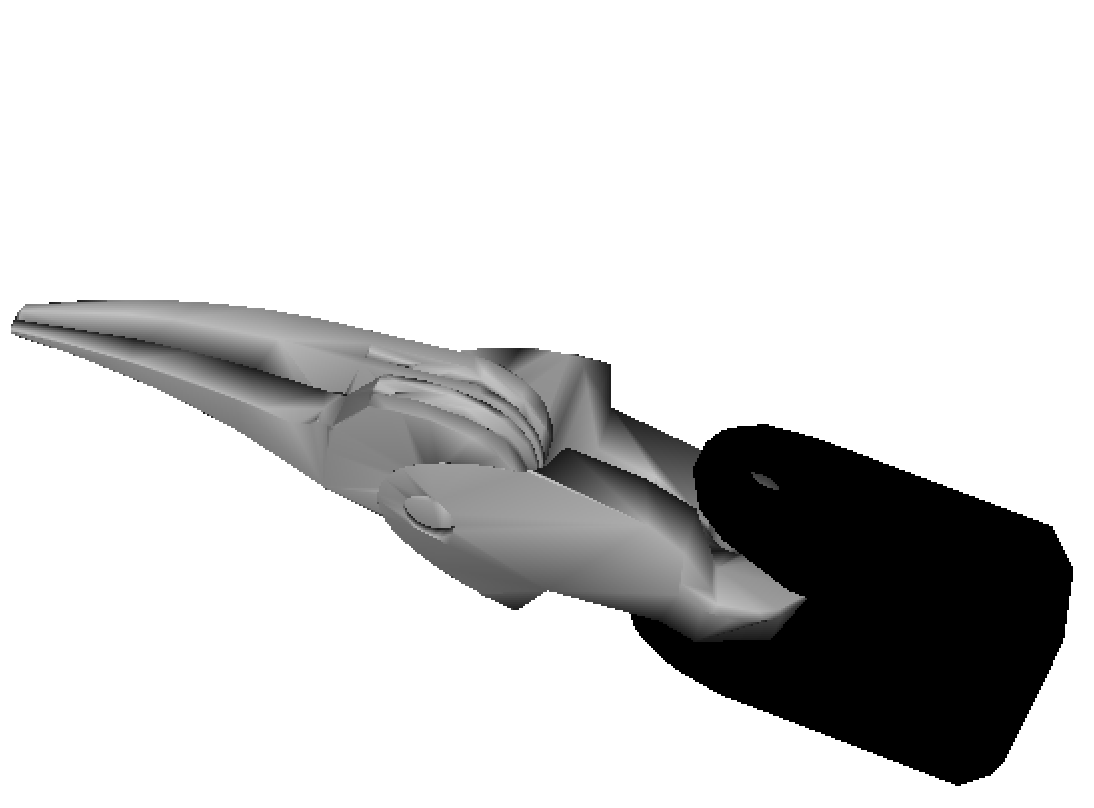
\includegraphics[width=0.35\linewidth]{integration/sofa_endowrist}
  \caption{---}\label{fig:sofa_endowrist}
\end{figure}

\subsection{Cutting}
Now we want to implement the cutting to simulate the dissection in a robotic surgery. To achieve this we had to use a SOFA plugin called SOFA Carving Plugin, which gave us the capability to cut a 3D mesh. The cutting was not as advanced as our cutting algorithm, instead it was doing the more basic and traditional way of cutting, which was simply deleting triangles and tetrahedra. We faced issues regarding the cutting in the scene that SOFA was limiting us to be only cutting one model, instead of multiple models, at the same time. In addition, the cutting tool was also limited to one model.

\begin{figure}
  \centering%
  
\includegraphics[width=0.35\linewidth]{integration/sofa_cloth}
  \caption{---}\label{fig:sofa_cloth}
\end{figure}

\subsection{Input Interface}
Finally, we worked on integrating the 3DSystems Touch with our SOFA program using another SOFA plugin. We first started with linking keyboard inputs through Python since SOFA allows the use of Python scripts to interact with its environment. Afterwards, we used a plugin provided by SOFA called Geomagic which is the same company that (used) to make the 3DSystem Touch (Omni Phantom) but it is developed by the SOFA team. The plugin gave us the capability of connecting the Touch to SOFA and moving the models using it.

\begin{figure}
  \centering%
  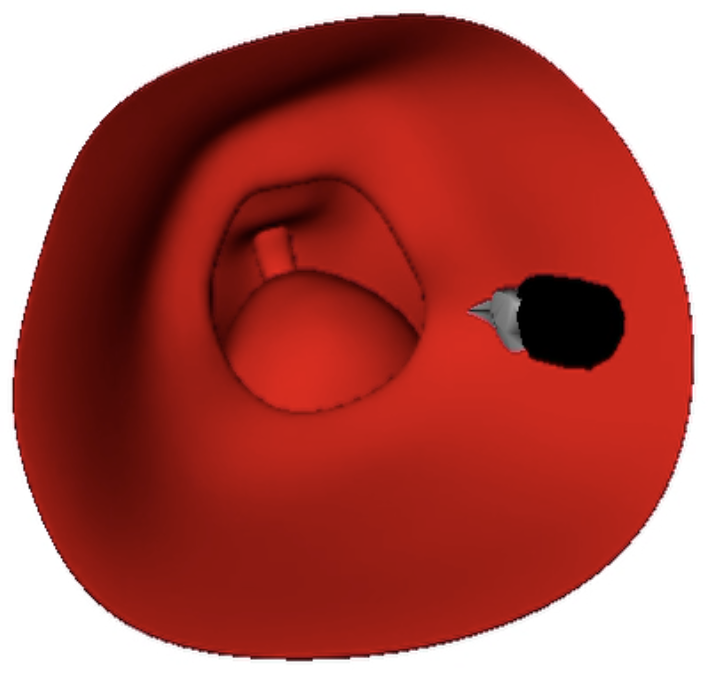
\includegraphics[width=0.5\linewidth]{integration/sofa_interaction}
  \caption{---}\label{fig:sofa_interaction}
\end{figure}

In conclusion, SOFA turned out to be a great choice for us to go with, given all its functionality, but it still has it is own hurdles which we need to work around.

\section{Scenarios Replay}\label{sec:replay}
Our logging module that was mainly developed for Aim 5 and 6, allows us to record the user's actions and replay them. This can be used to recored multiple scenarios and to monitor a user's progress.


\begin{figure}
  \centering%
  \setlength{\fboxsep}{0pt}%
  \setlength{\fboxrule}{0.1pt}%
  \fbox{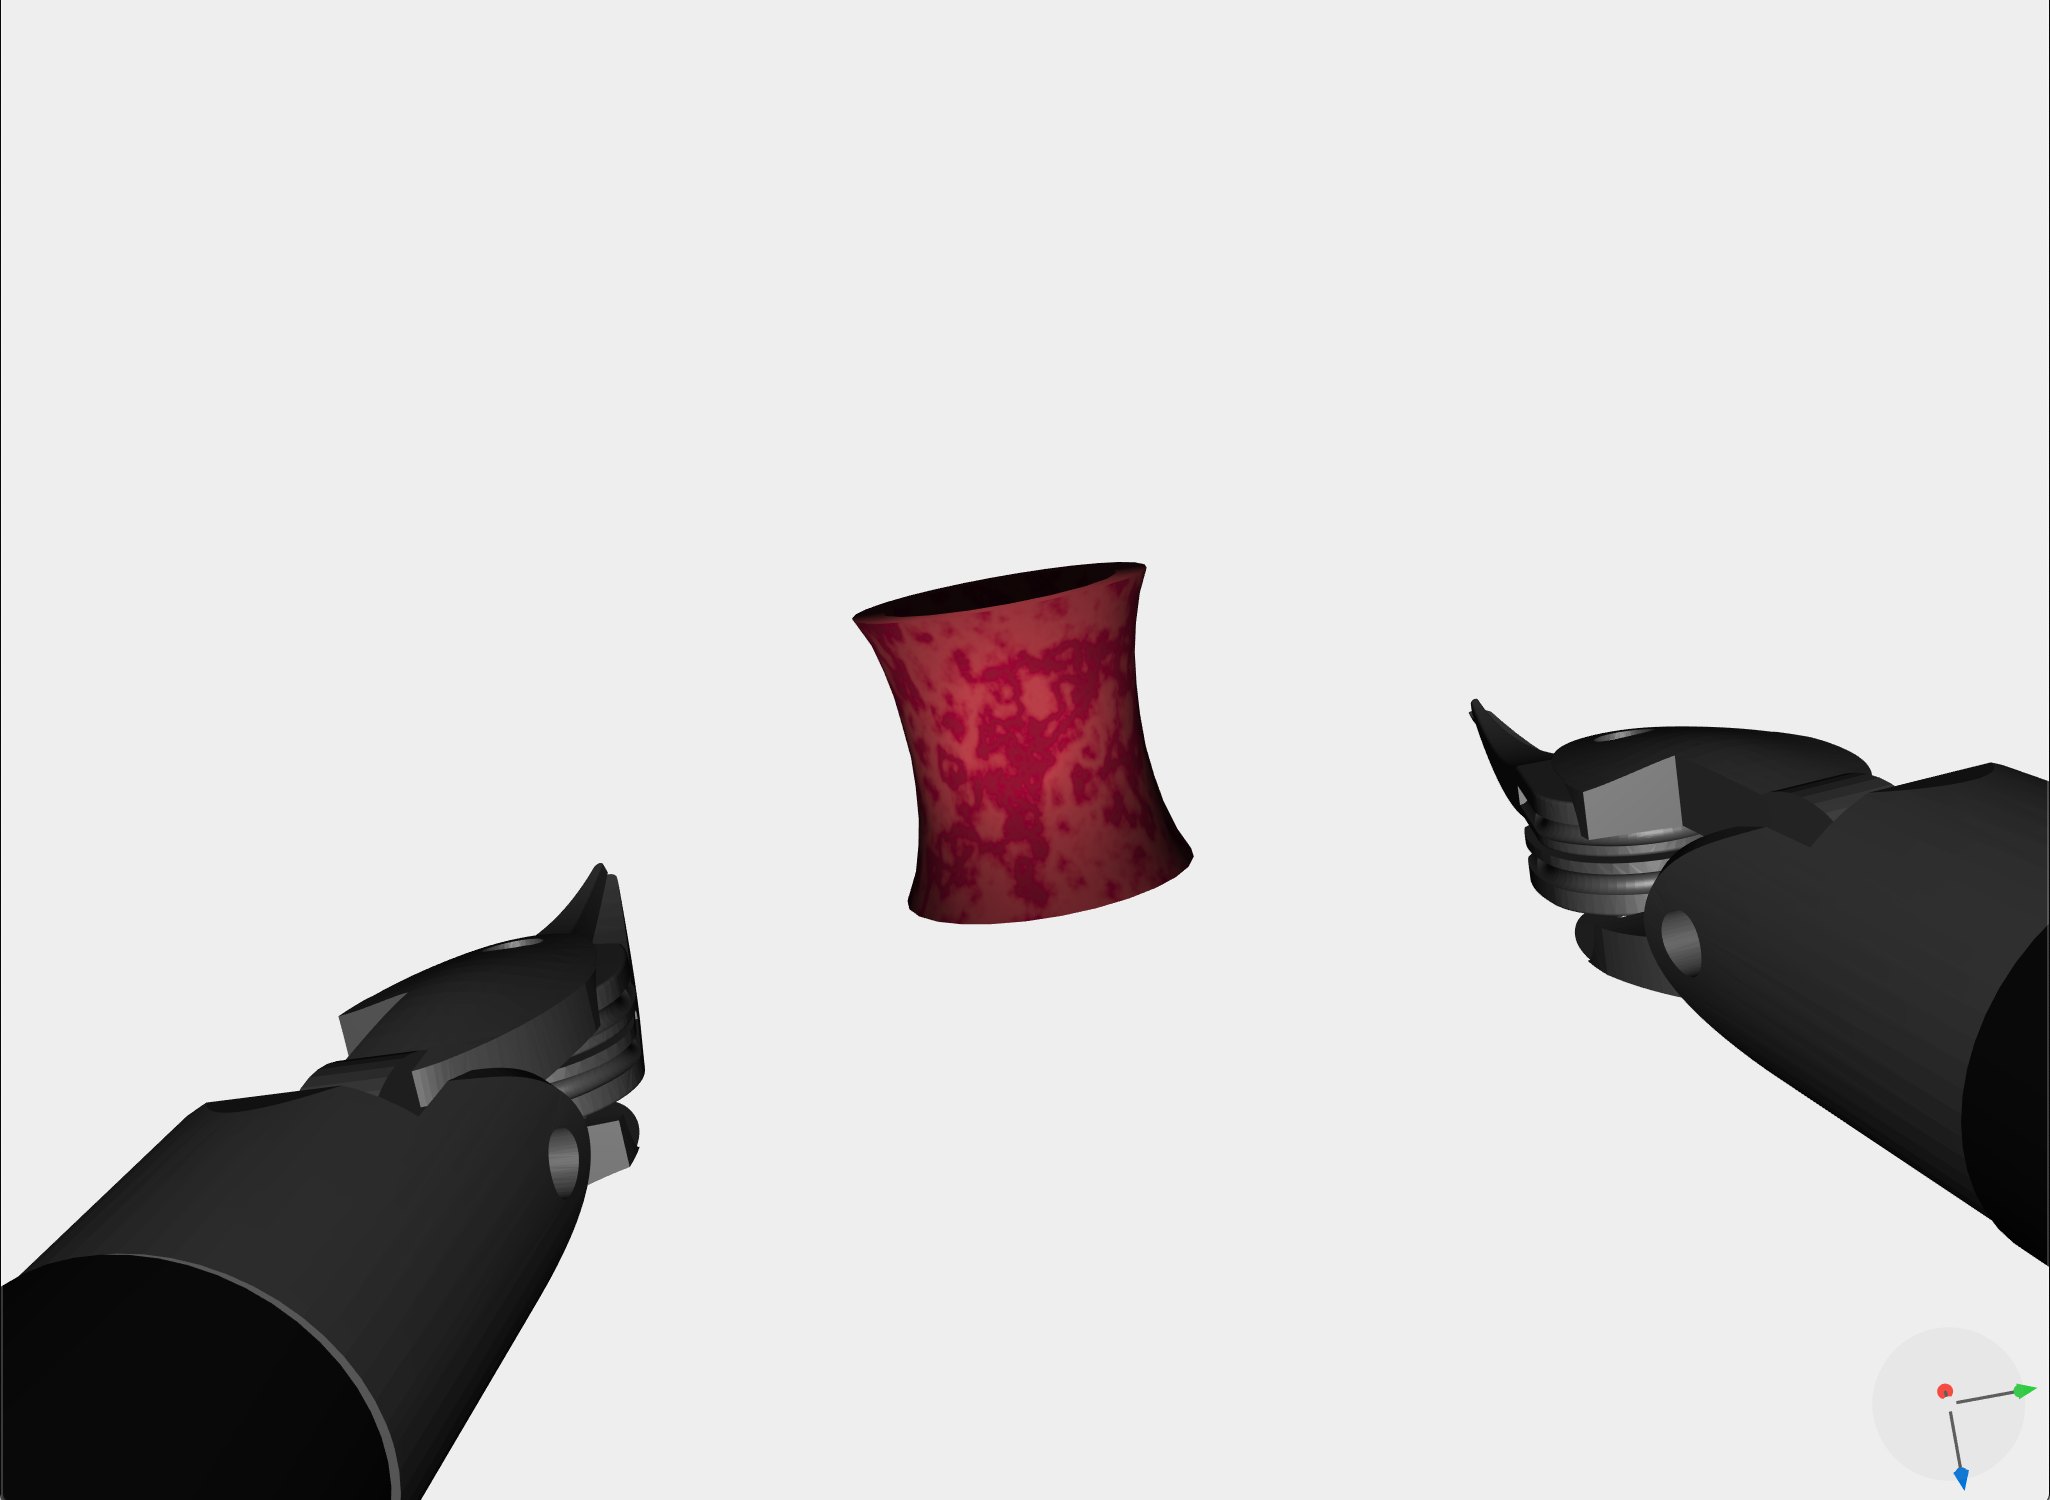
\includegraphics[width=0.49\linewidth]{integration/snap0}}\hfill%
  \fbox{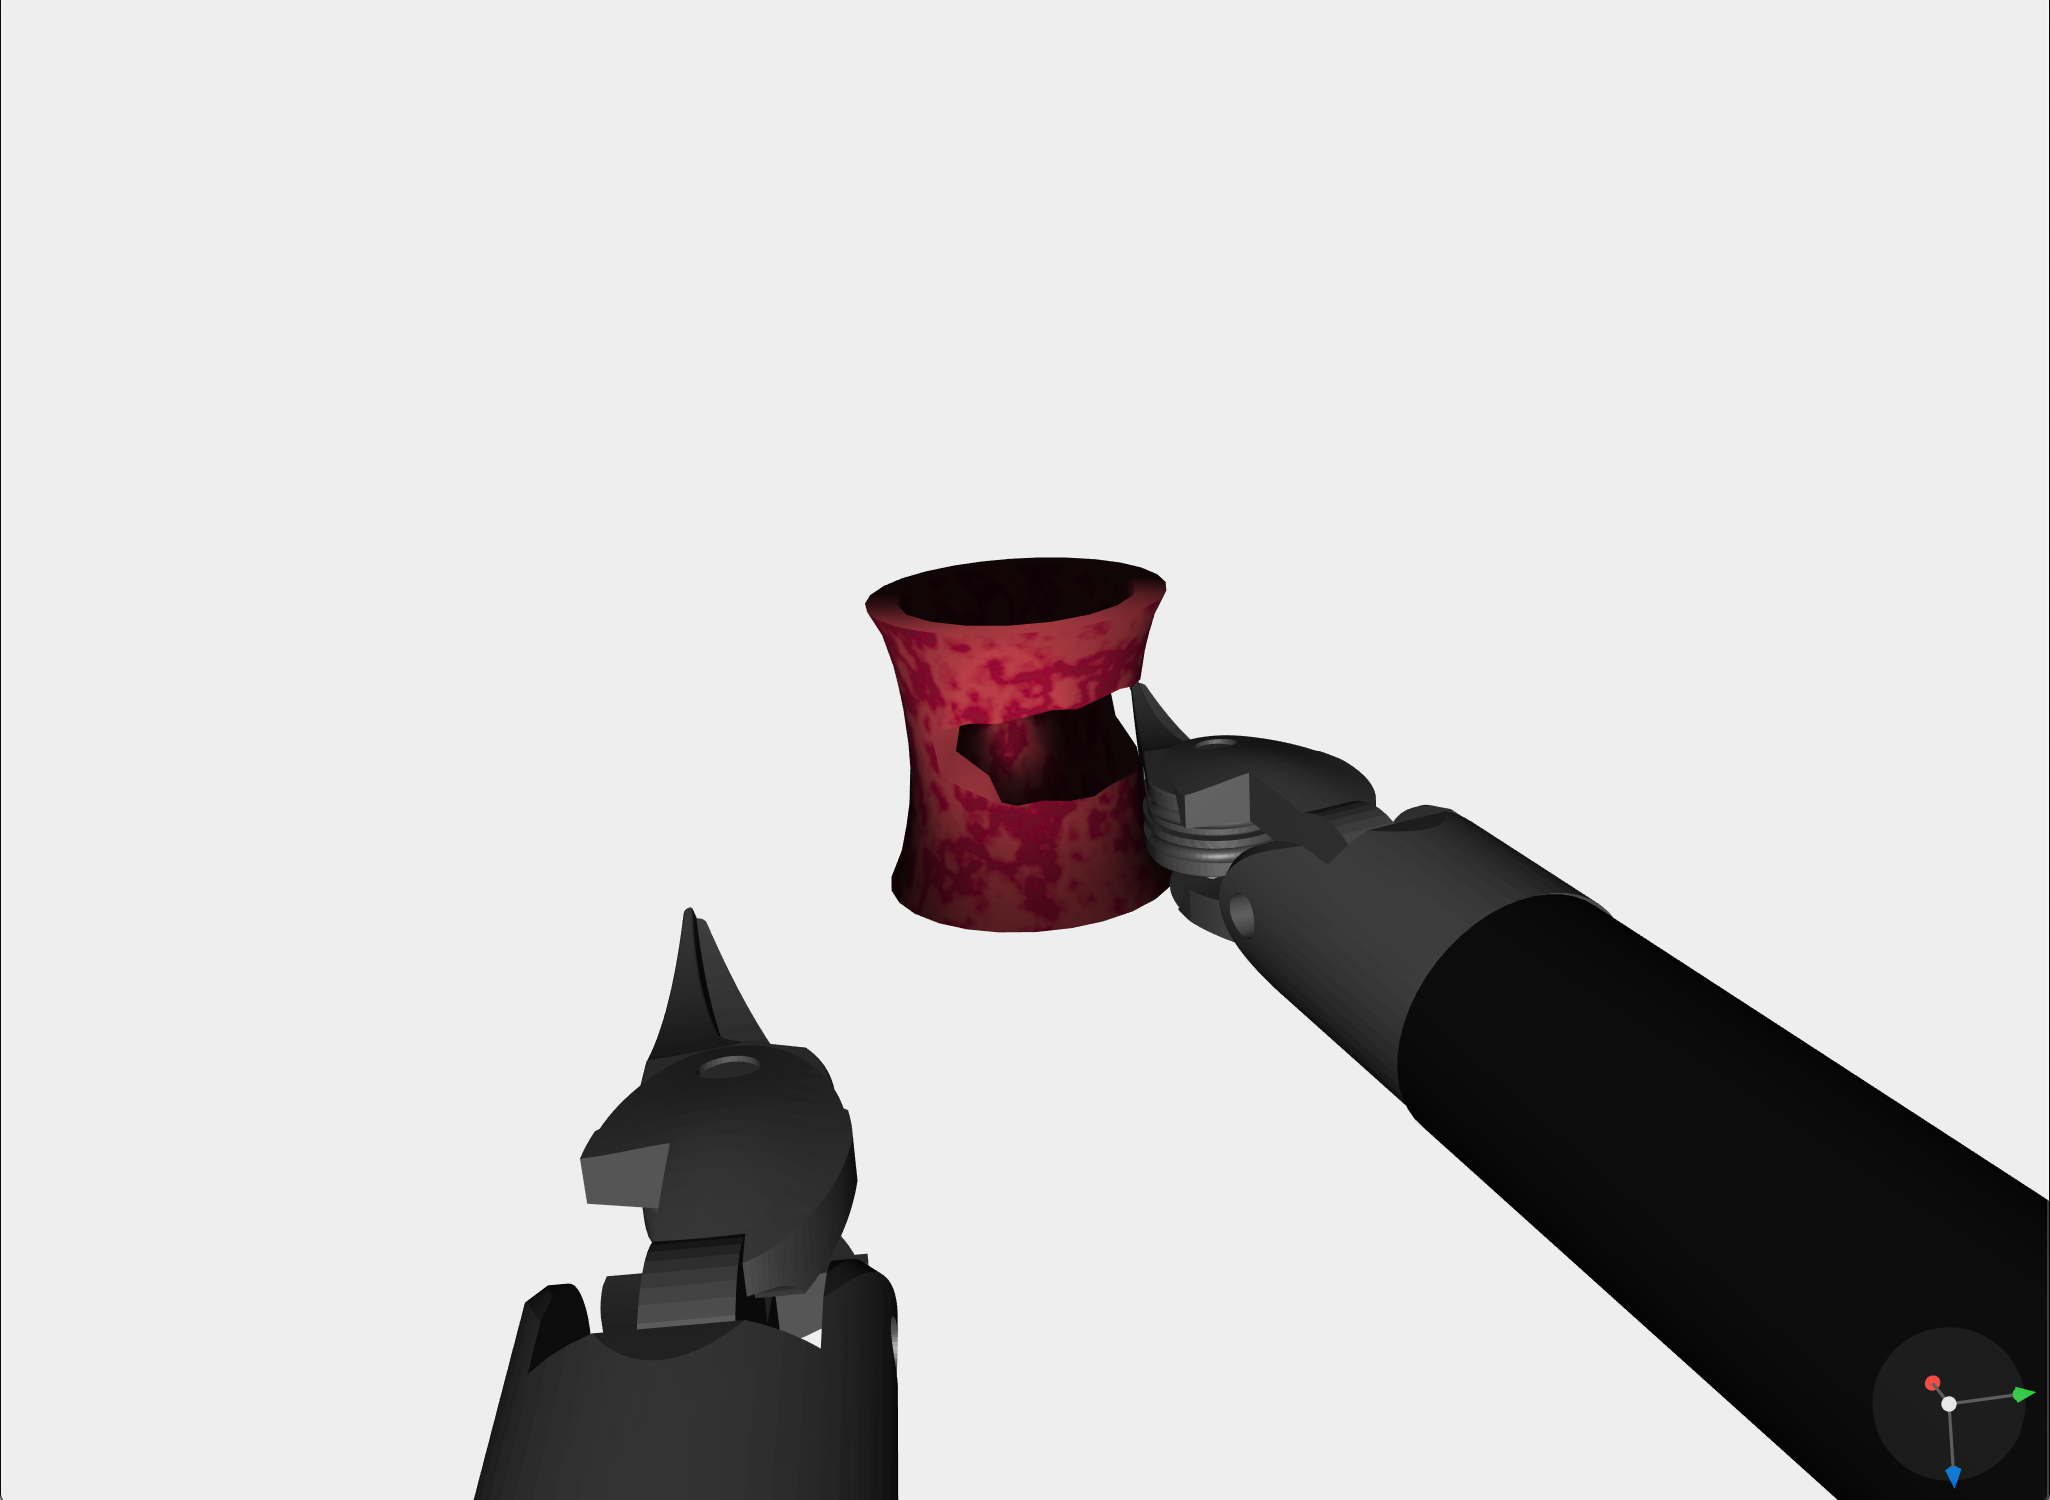
\includegraphics[width=0.49\linewidth]{integration/snap1}}\\[1.5ex]%
  \fbox{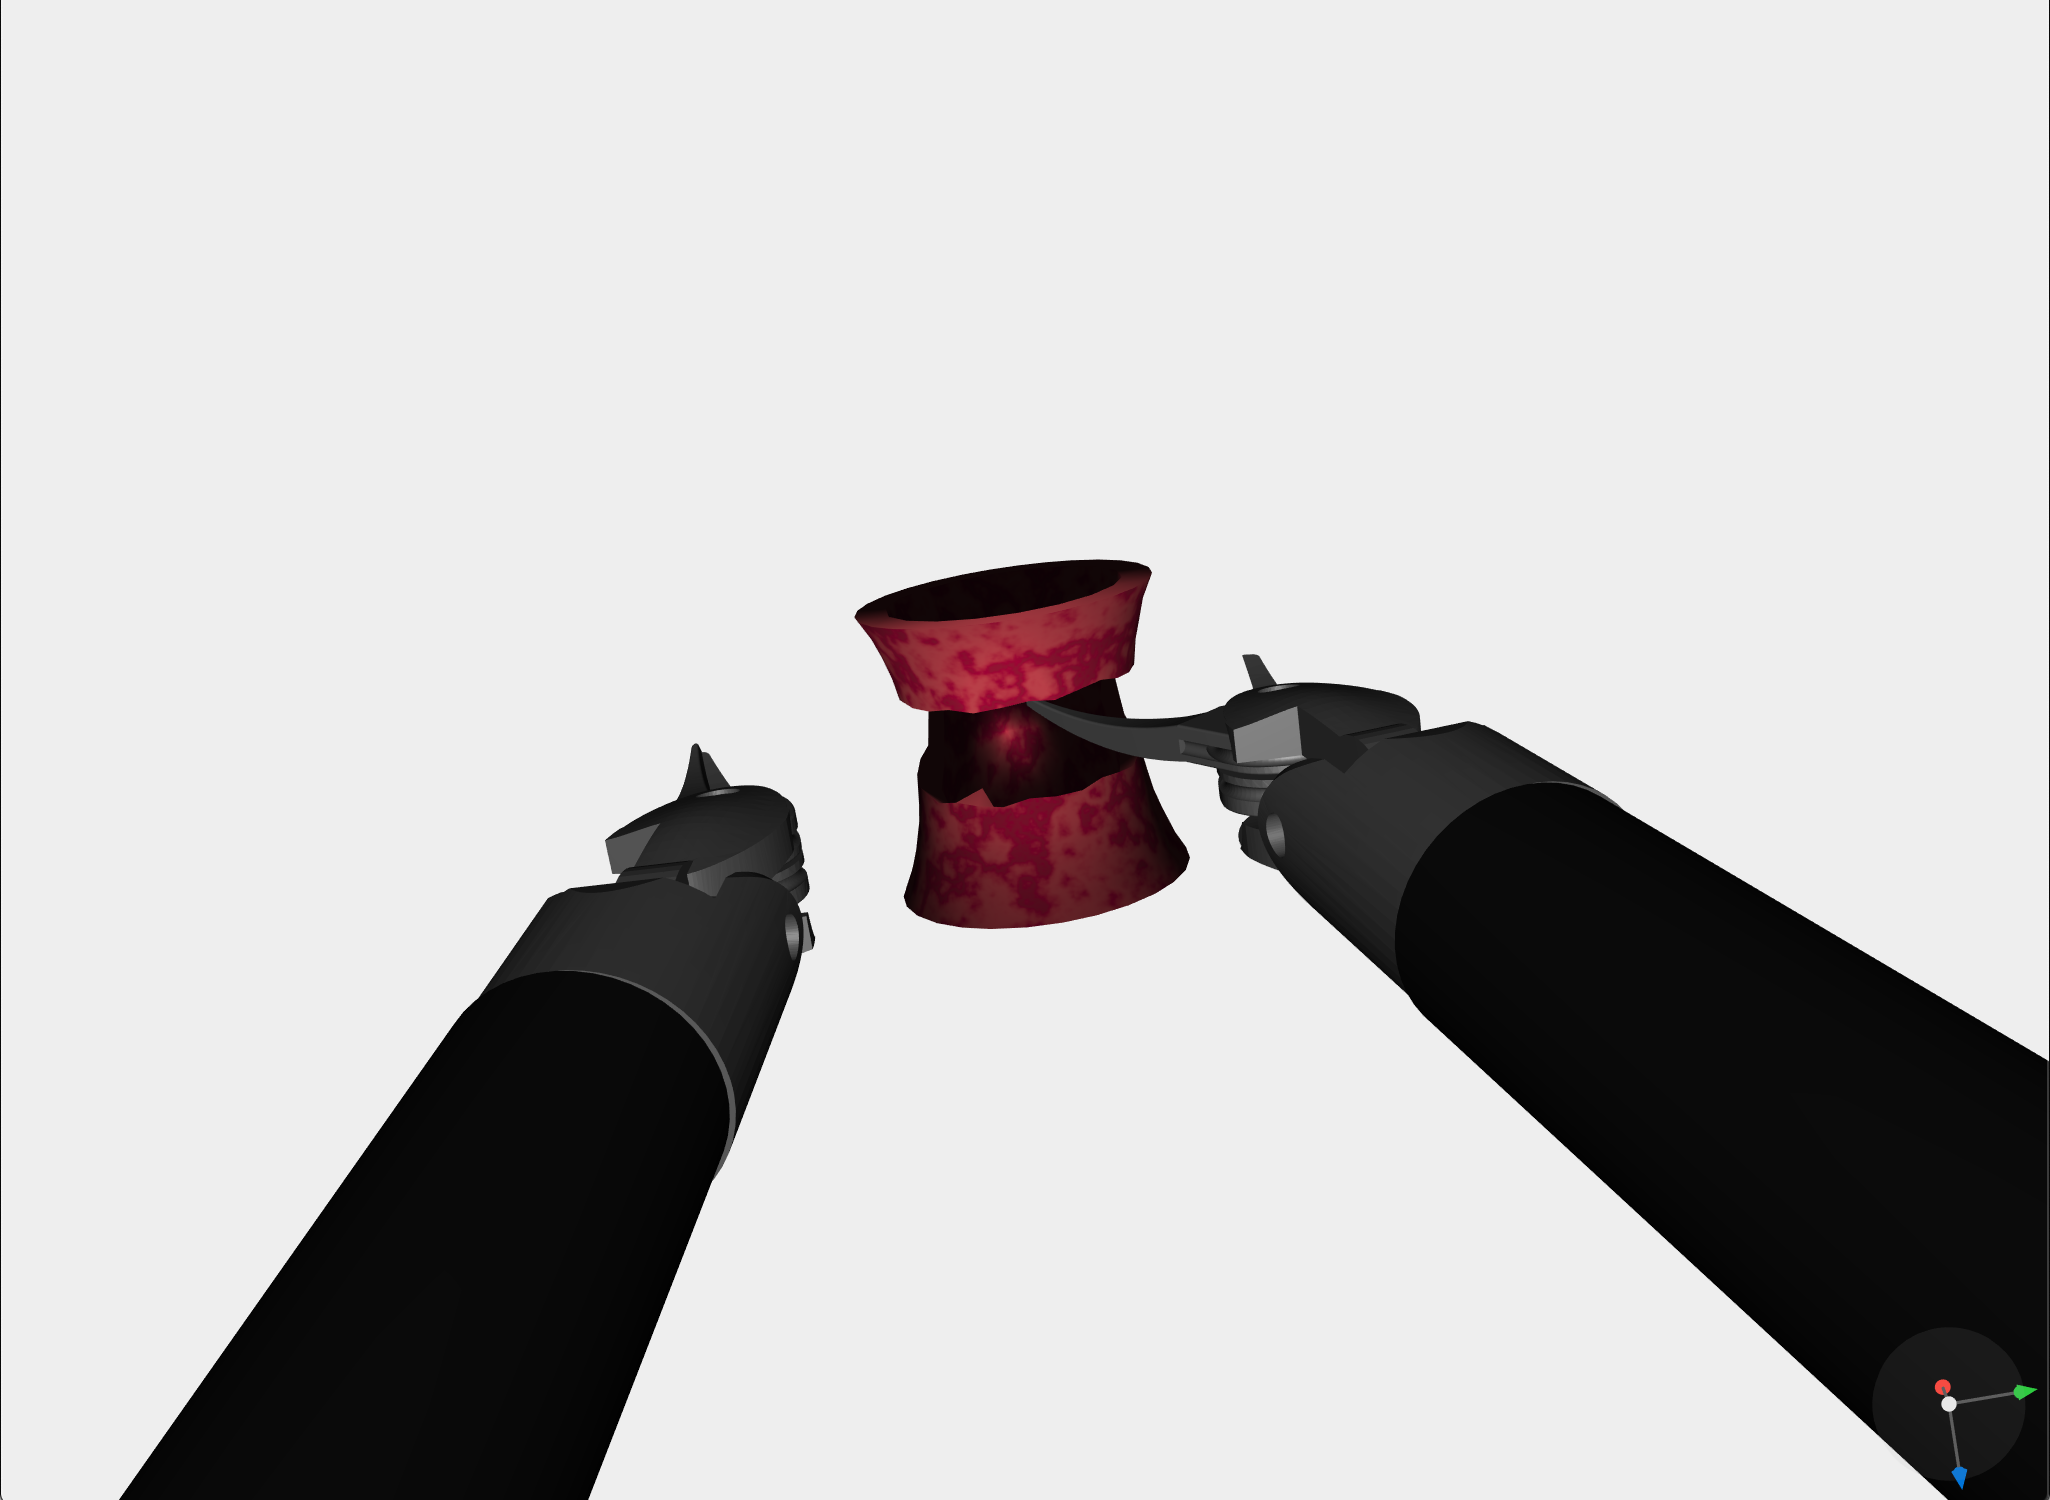
\includegraphics[width=0.49\linewidth]{integration/snap2}}\hfill%
  \fbox{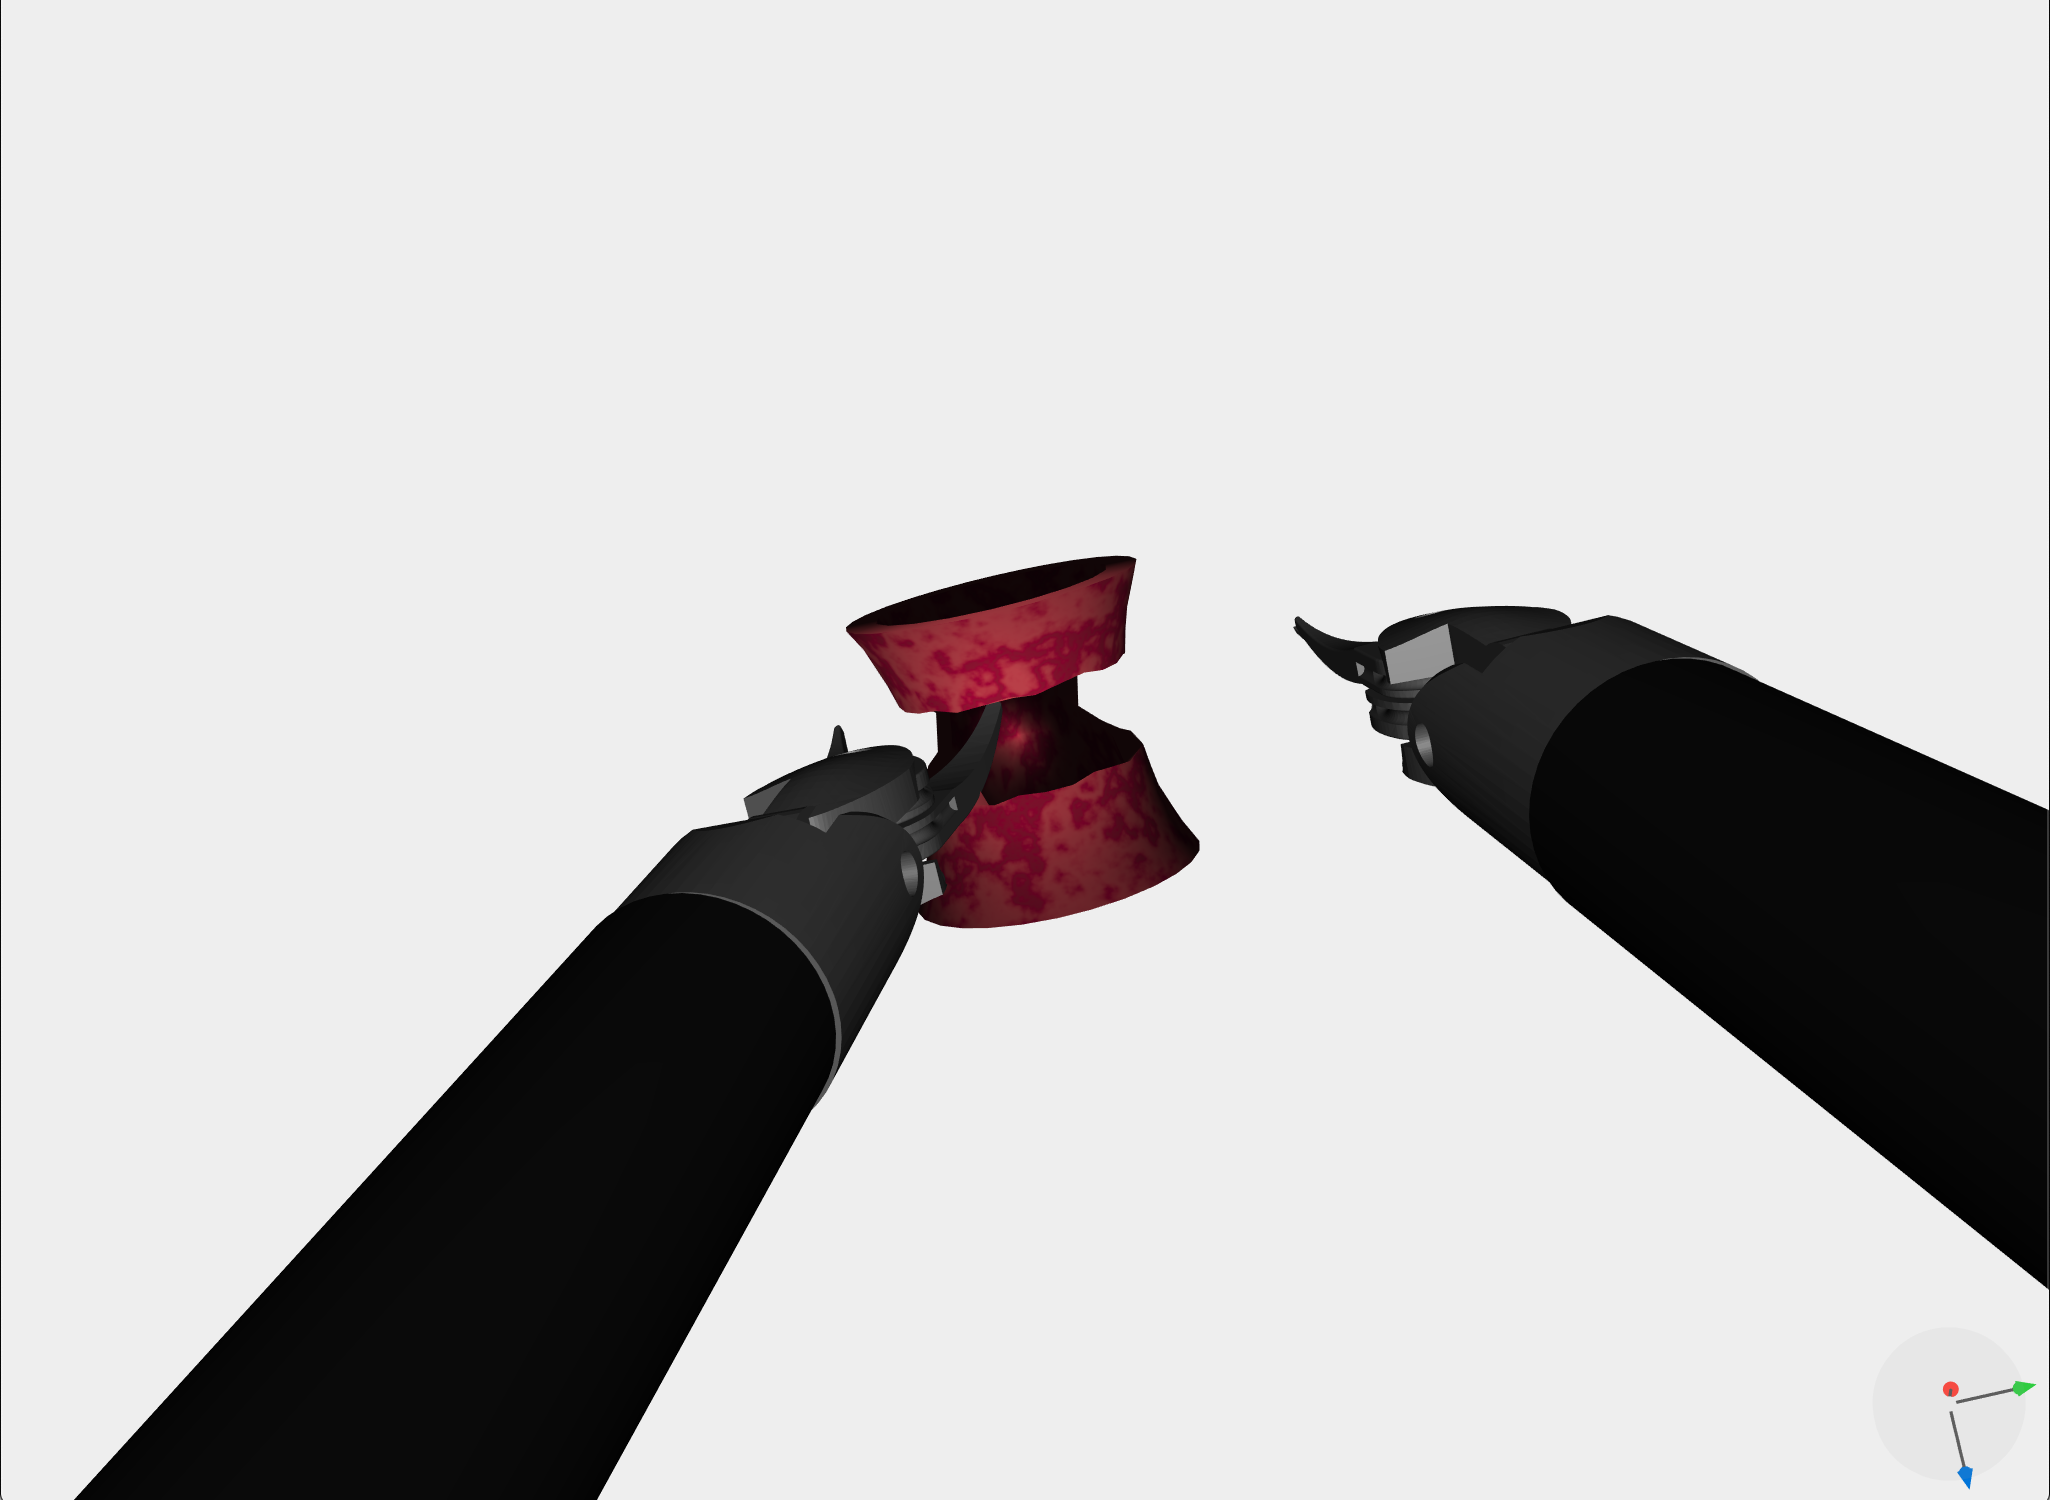
\includegraphics[width=0.49\linewidth]{integration/snap3}}\\[1.5ex]%
  \fbox{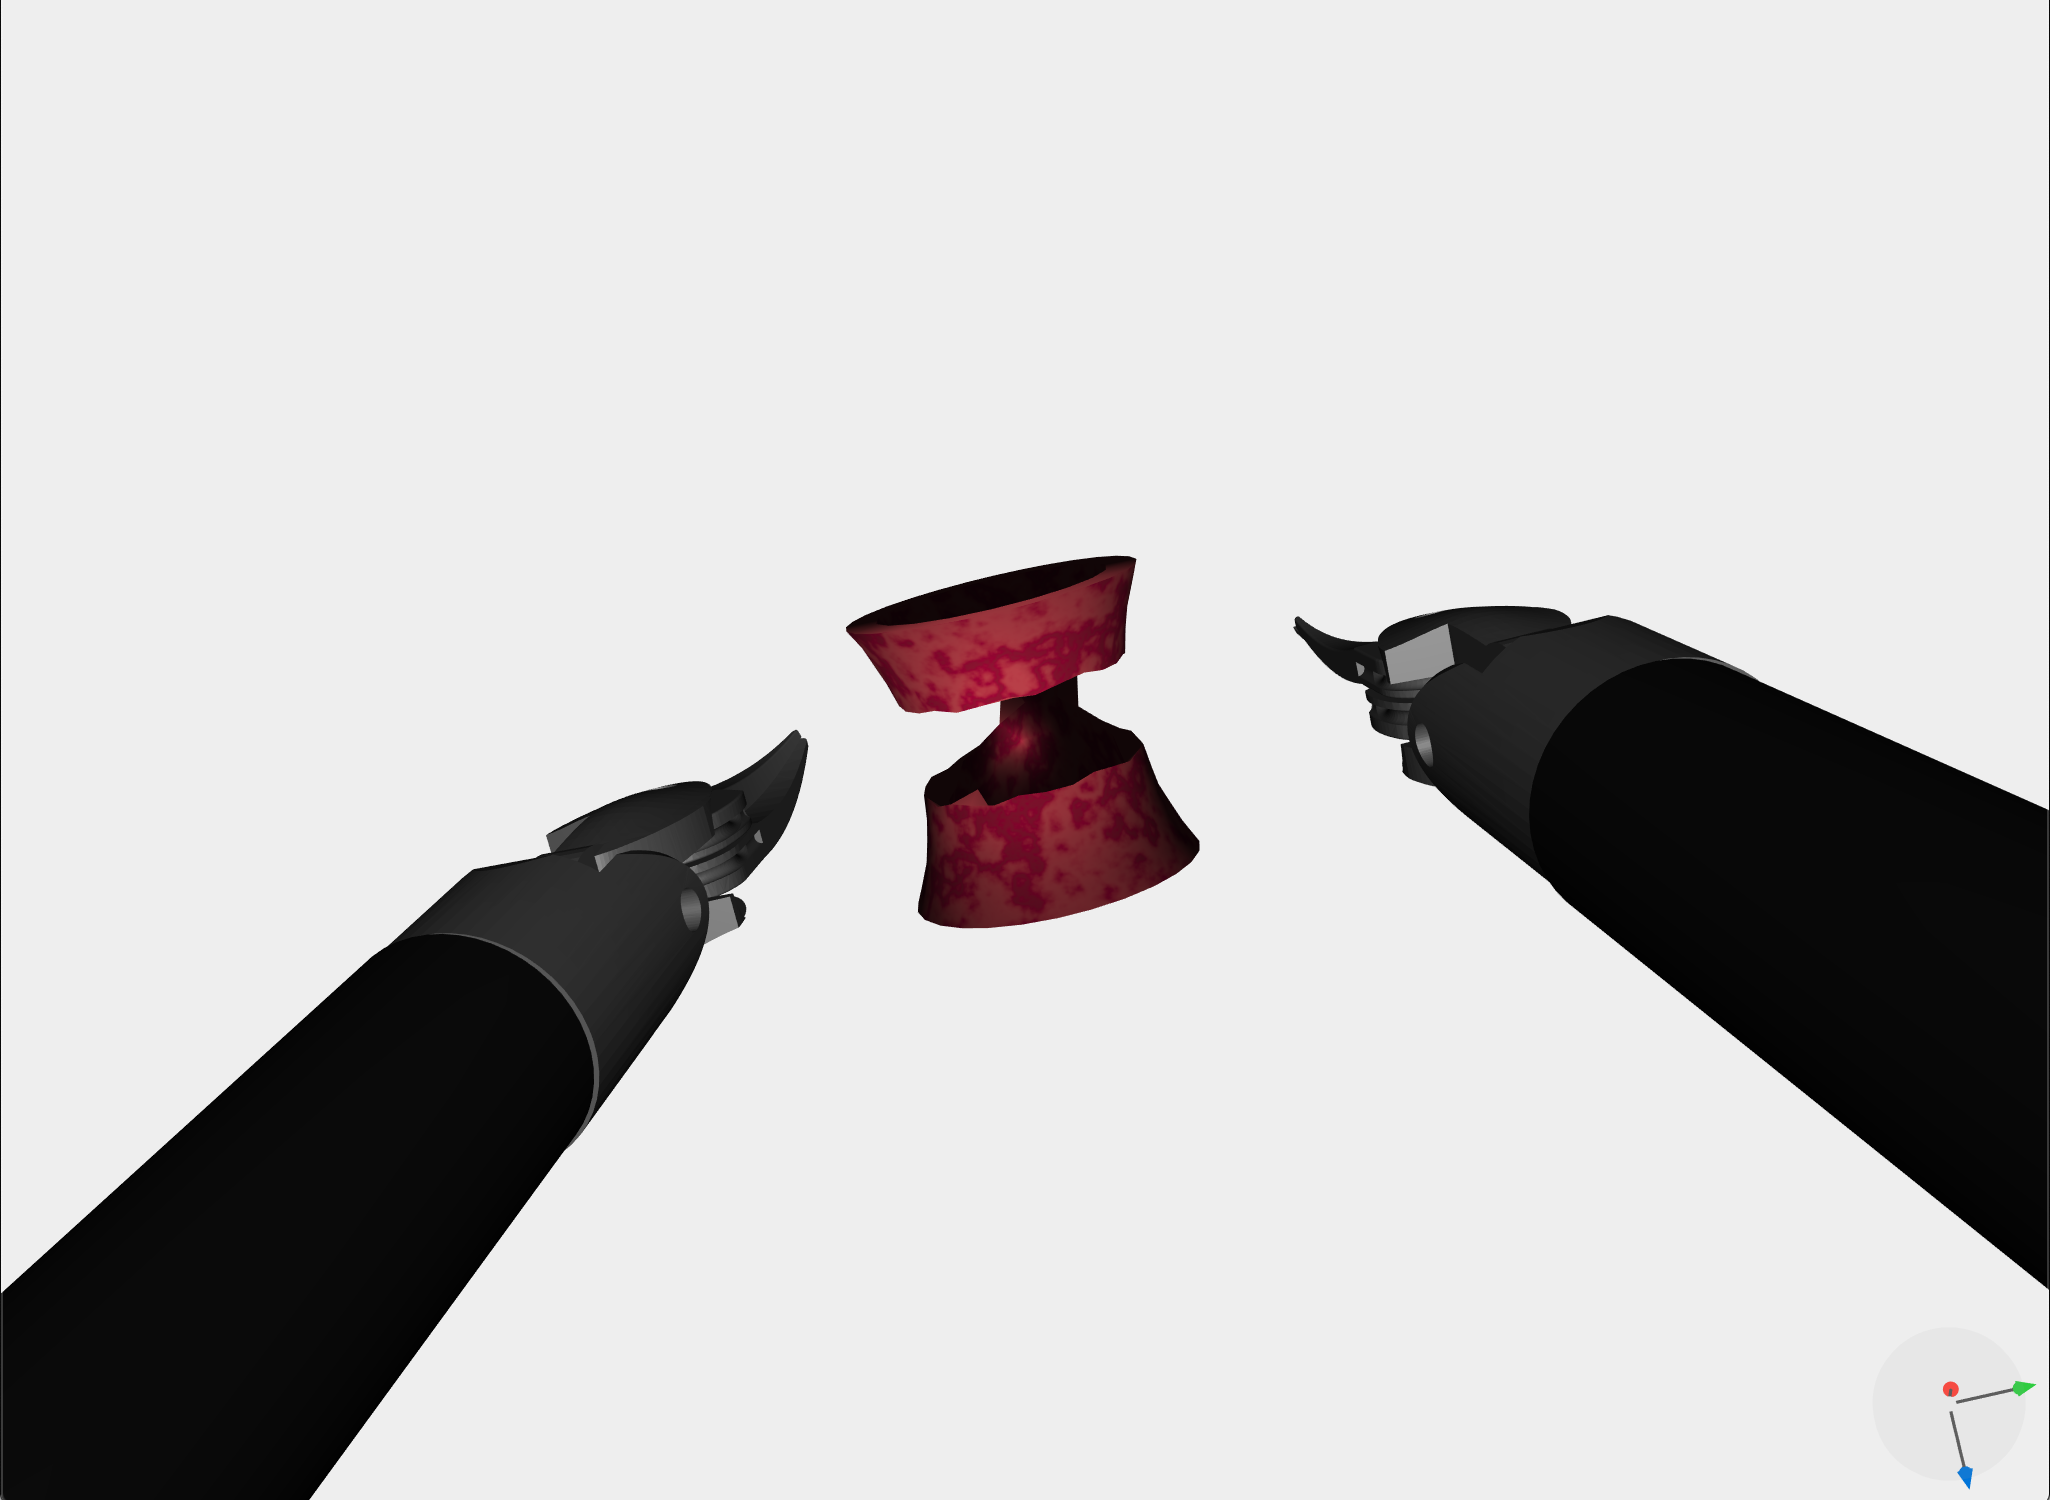
\includegraphics[width=0.49\linewidth]{integration/snap4}}\hfill%
  \fbox{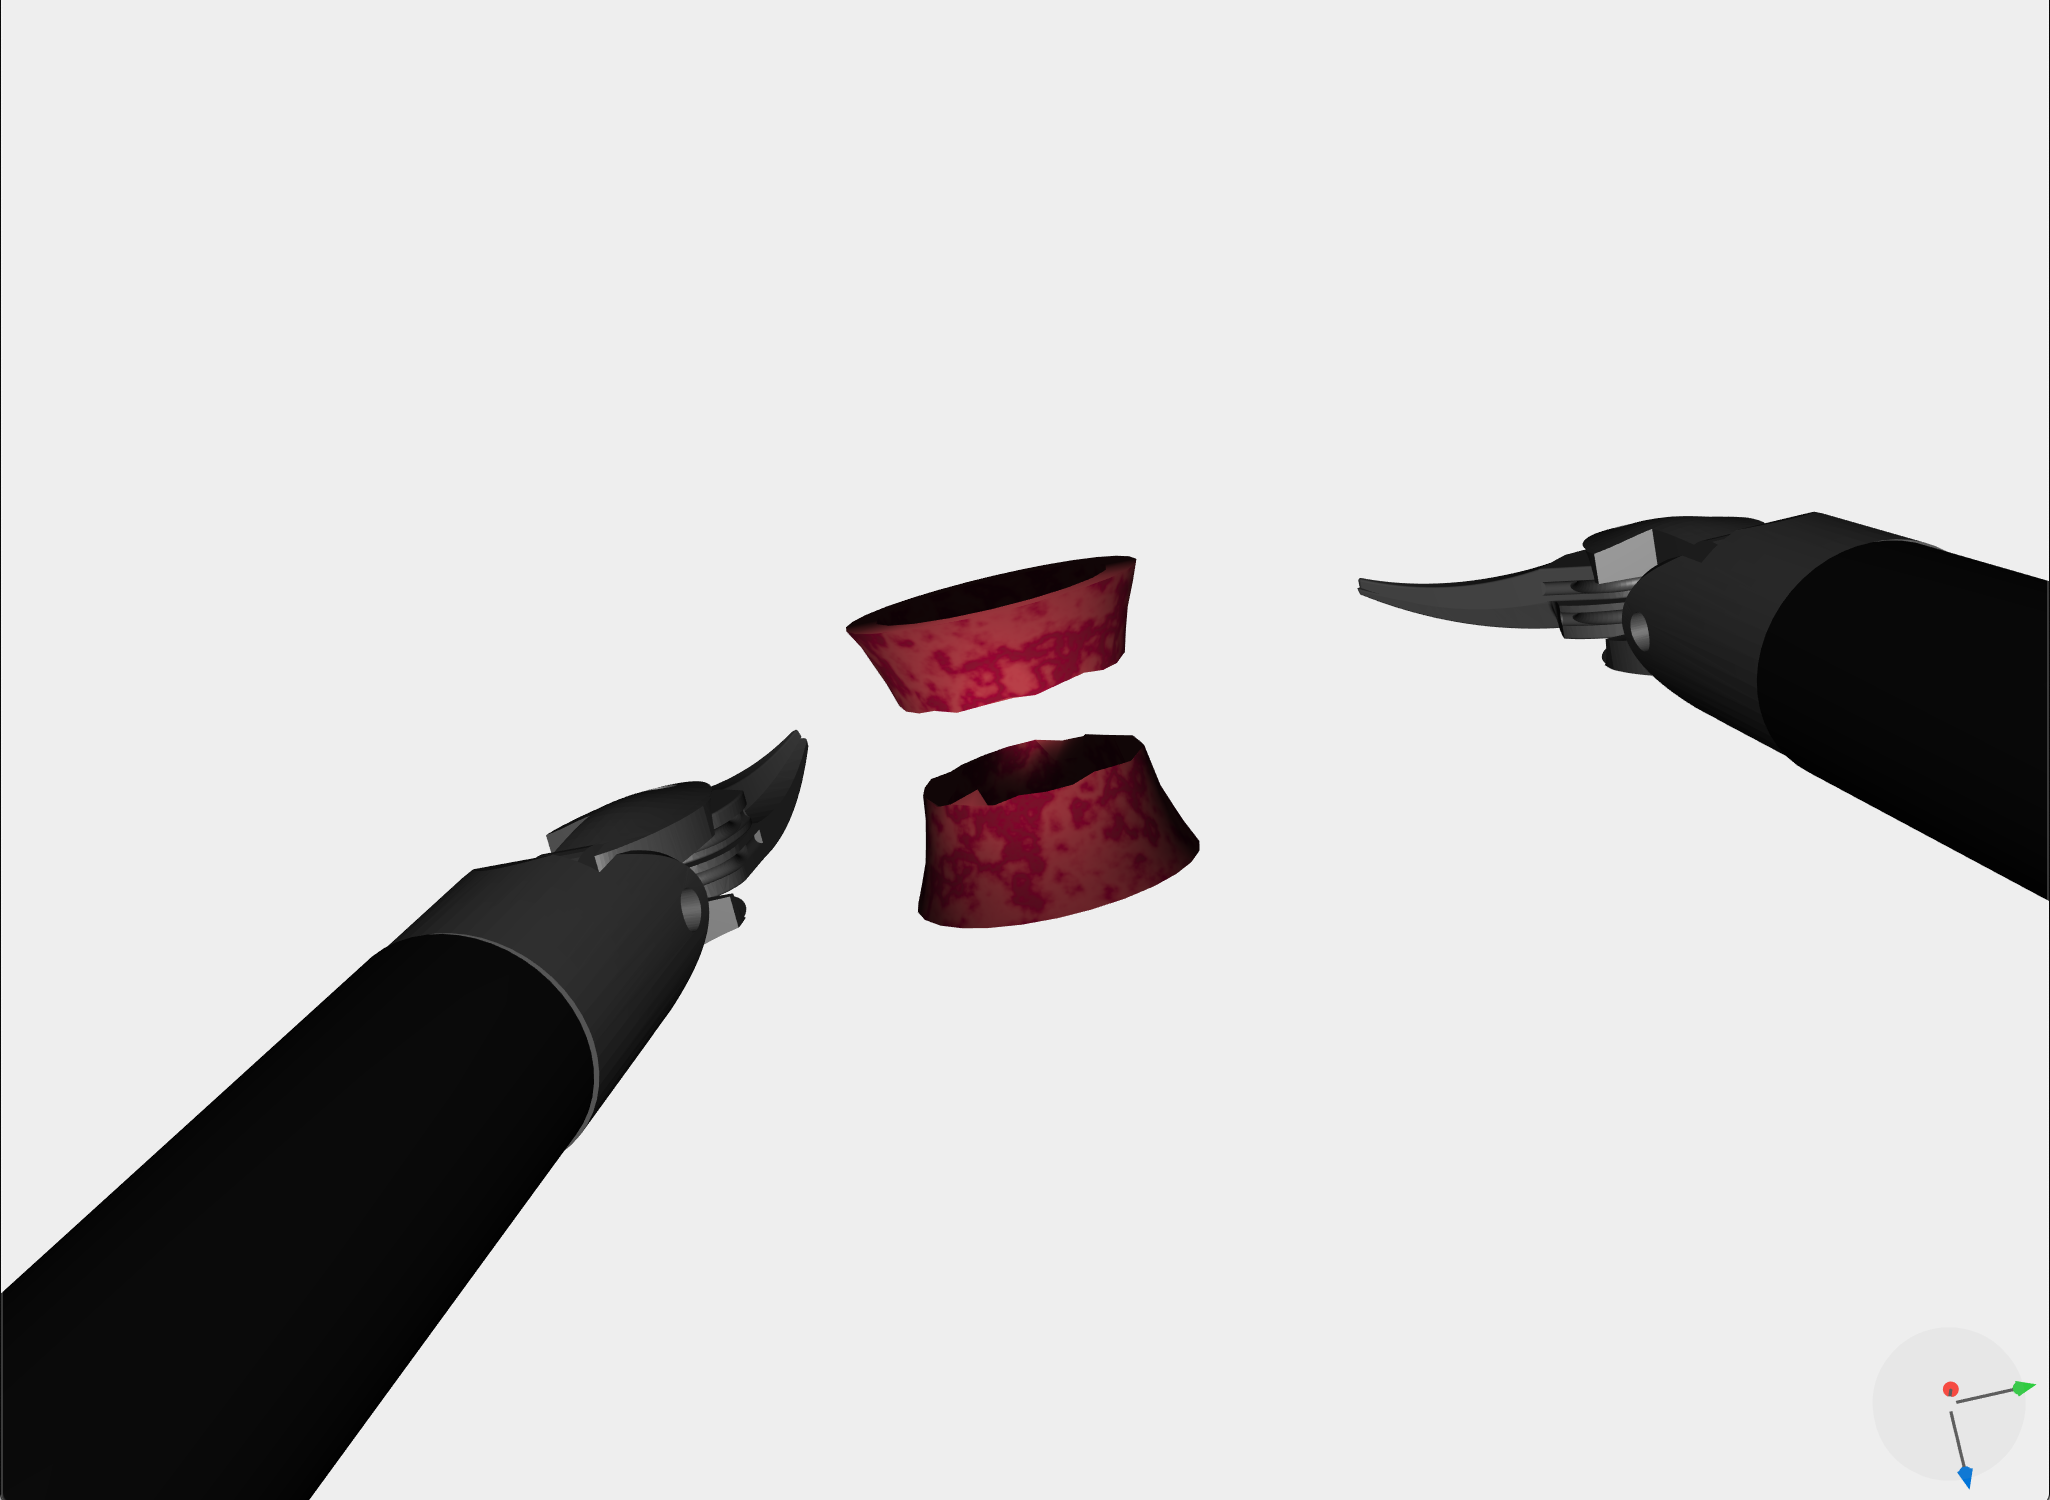
\includegraphics[width=0.49\linewidth]{integration/snap5}}\\[1.5ex]%
  \caption{---}\label{fig:cuts}
\end{figure}

\hrule%

\clearpage%
